\documentclass[twoside]{book}

% Packages required by doxygen
\usepackage{calc}
\usepackage{doxygen}
\usepackage{graphicx}
\usepackage[utf8]{inputenc}
\usepackage{makeidx}
\usepackage{multicol}
\usepackage{multirow}
\usepackage{textcomp}
\usepackage[table]{xcolor}

% Font selection
\usepackage[T1]{fontenc}
\usepackage{mathptmx}
\usepackage[scaled=.90]{helvet}
\usepackage{courier}
\usepackage{amssymb}
\usepackage{sectsty}
\renewcommand{\familydefault}{\sfdefault}
\allsectionsfont{%
  \fontseries{bc}\selectfont%
  \color{darkgray}%
}
\renewcommand{\DoxyLabelFont}{%
  \fontseries{bc}\selectfont%
  \color{darkgray}%
}

% Page & text layout
\usepackage{geometry}
\geometry{%
  a4paper,%
  top=2.5cm,%
  bottom=2.5cm,%
  left=2.5cm,%
  right=2.5cm%
}
\tolerance=750
\hfuzz=15pt
\hbadness=750
\setlength{\emergencystretch}{15pt}
\setlength{\parindent}{0cm}
\setlength{\parskip}{0.2cm}
\makeatletter
\renewcommand{\paragraph}{%
  \@startsection{paragraph}{4}{0ex}{-1.0ex}{1.0ex}{%
    \normalfont\normalsize\bfseries\SS@parafont%
  }%
}
\renewcommand{\subparagraph}{%
  \@startsection{subparagraph}{5}{0ex}{-1.0ex}{1.0ex}{%
    \normalfont\normalsize\bfseries\SS@subparafont%
  }%
}
\makeatother

% Headers & footers
\usepackage{fancyhdr}
\pagestyle{fancyplain}
\fancyhead[LE]{\fancyplain{}{\bfseries\thepage}}
\fancyhead[CE]{\fancyplain{}{}}
\fancyhead[RE]{\fancyplain{}{\bfseries\leftmark}}
\fancyhead[LO]{\fancyplain{}{\bfseries\rightmark}}
\fancyhead[CO]{\fancyplain{}{}}
\fancyhead[RO]{\fancyplain{}{\bfseries\thepage}}
\fancyfoot[LE]{\fancyplain{}{}}
\fancyfoot[CE]{\fancyplain{}{}}
\fancyfoot[RE]{\fancyplain{}{\bfseries\scriptsize Generated on Wed Aug 28 2013 22\-:19\-:22 for B\-M\-E.\-Core by Doxygen }}
\fancyfoot[LO]{\fancyplain{}{\bfseries\scriptsize Generated on Wed Aug 28 2013 22\-:19\-:22 for B\-M\-E.\-Core by Doxygen }}
\fancyfoot[CO]{\fancyplain{}{}}
\fancyfoot[RO]{\fancyplain{}{}}
\renewcommand{\footrulewidth}{0.4pt}
\renewcommand{\chaptermark}[1]{%
  \markboth{#1}{}%
}
\renewcommand{\sectionmark}[1]{%
  \markright{\thesection\ #1}%
}

% Indices & bibliography
\usepackage{natbib}
\usepackage[titles]{tocloft}
\setcounter{tocdepth}{3}
\setcounter{secnumdepth}{5}
\makeindex

% Hyperlinks (required, but should be loaded last)
\usepackage{ifpdf}
\ifpdf
  \usepackage[pdftex,pagebackref=true]{hyperref}
\else
  \usepackage[ps2pdf,pagebackref=true]{hyperref}
\fi
\hypersetup{%
  colorlinks=true,%
  linkcolor=blue,%
  citecolor=blue,%
  unicode%
}

% Custom commands
\newcommand{\clearemptydoublepage}{%
  \newpage{\pagestyle{empty}\cleardoublepage}%
}


%===== C O N T E N T S =====

\begin{document}

% Titlepage & ToC
\hypersetup{pageanchor=false}
\pagenumbering{roman}
\begin{titlepage}
\vspace*{7cm}
\begin{center}%
{\Large B\-M\-E.\-Core \\[1ex]\large 1.\-0 }\\
\vspace*{1cm}
{\large Generated by Doxygen 1.8.5}\\
\vspace*{0.5cm}
{\small Wed Aug 28 2013 22:19:22}\\
\end{center}
\end{titlepage}
\clearemptydoublepage
\tableofcontents
\clearemptydoublepage
\pagenumbering{arabic}
\hypersetup{pageanchor=true}

%--- Begin generated contents ---
\chapter{Namespace Index}
\section{Packages}
Here are the packages with brief descriptions (if available)\-:\begin{DoxyCompactList}
\item\contentsline{section}{\hyperlink{namespace_b_m_s}{B\-M\-S} }{\pageref{namespace_b_m_s}}{}
\item\contentsline{section}{\hyperlink{namespace_b_m_s_1_1_core}{B\-M\-S.\-Core} }{\pageref{namespace_b_m_s_1_1_core}}{}
\end{DoxyCompactList}

\chapter{Hierarchical Index}
\section{Class Hierarchy}
This inheritance list is sorted roughly, but not completely, alphabetically\-:\begin{DoxyCompactList}
\item \contentsline{section}{B\-M\-S.\-Core.\-B\-M\-S\-\_\-\-Log\-Factory}{\pageref{class_b_m_s_1_1_core_1_1_b_m_s___log_factory}}{}
\begin{DoxyCompactList}
\item \contentsline{section}{B\-M\-S.\-Core.\-B\-M\-S\-\_\-\-File\-Log\-Factory}{\pageref{class_b_m_s_1_1_core_1_1_b_m_s___file_log_factory}}{}
\end{DoxyCompactList}
\item \contentsline{section}{B\-M\-S.\-Core.\-B\-M\-S\-\_\-\-Logger}{\pageref{class_b_m_s_1_1_core_1_1_b_m_s___logger}}{}
\begin{DoxyCompactList}
\item \contentsline{section}{B\-M\-S.\-Core.\-B\-M\-S\-\_\-\-File\-Logger}{\pageref{class_b_m_s_1_1_core_1_1_b_m_s___file_logger}}{}
\end{DoxyCompactList}
\end{DoxyCompactList}

\chapter{Class Index}
\section{Class List}
Here are the classes, structs, unions and interfaces with brief descriptions\-:\begin{DoxyCompactList}
\item\contentsline{section}{\hyperlink{class_b_m_s_1_1_core_1_1_b_m_s___file_log_factory}{B\-M\-S.\-Core.\-B\-M\-S\-\_\-\-File\-Log\-Factory} }{\pageref{class_b_m_s_1_1_core_1_1_b_m_s___file_log_factory}}{}
\item\contentsline{section}{\hyperlink{class_b_m_s_1_1_core_1_1_b_m_s___file_logger}{B\-M\-S.\-Core.\-B\-M\-S\-\_\-\-File\-Logger} }{\pageref{class_b_m_s_1_1_core_1_1_b_m_s___file_logger}}{}
\item\contentsline{section}{\hyperlink{class_b_m_s_1_1_core_1_1_b_m_s___log_factory}{B\-M\-S.\-Core.\-B\-M\-S\-\_\-\-Log\-Factory} \\*Abstract base class for all \hyperlink{class_b_m_s_1_1_core_1_1_b_m_s___log_factory}{B\-M\-S\-\_\-\-Log\-Factory} implementations. Provides interface methods. }{\pageref{class_b_m_s_1_1_core_1_1_b_m_s___log_factory}}{}
\item\contentsline{section}{\hyperlink{class_b_m_s_1_1_core_1_1_b_m_s___logger}{B\-M\-S.\-Core.\-B\-M\-S\-\_\-\-Logger} \\*Abstract base class for all \hyperlink{class_b_m_s_1_1_core_1_1_b_m_s___logger}{B\-M\-S\-\_\-\-Logger} implementations. Provides interface details and common members as well as current logger containers. }{\pageref{class_b_m_s_1_1_core_1_1_b_m_s___logger}}{}
\end{DoxyCompactList}

\chapter{File Index}
\section{File List}
Here is a list of all files with brief descriptions\-:\begin{DoxyCompactList}
\item\contentsline{section}{E\-:/\-Projects/\-Bad Monkey Software/\-Software/\-B\-M\-E/\-Core/\hyperlink{_b_m_s___file_logger_8cs}{B\-M\-S\-\_\-\-File\-Logger.\-cs} }{\pageref{_b_m_s___file_logger_8cs}}{}
\item\contentsline{section}{E\-:/\-Projects/\-Bad Monkey Software/\-Software/\-B\-M\-E/\-Core/\hyperlink{_b_m_s___logger_8cs}{B\-M\-S\-\_\-\-Logger.\-cs} }{\pageref{_b_m_s___logger_8cs}}{}
\item\contentsline{section}{E\-:/\-Projects/\-Bad Monkey Software/\-Software/\-B\-M\-E/\-Core/obj/\-Debug Documented/\hyperlink{_debug_01_documented_2_temporary_generated_file__036_c0_b5_b-1481-4323-8_d20-8_f5_a_d_c_b23_d92_8cs}{Temporary\-Generated\-File\-\_\-036\-C0\-B5\-B-\/1481-\/4323-\/8\-D20-\/8\-F5\-A\-D\-C\-B23\-D92.\-cs} }{\pageref{_debug_01_documented_2_temporary_generated_file__036_c0_b5_b-1481-4323-8_d20-8_f5_a_d_c_b23_d92_8cs}}{}
\item\contentsline{section}{E\-:/\-Projects/\-Bad Monkey Software/\-Software/\-B\-M\-E/\-Core/obj/\-Debug Documented/\hyperlink{_debug_01_documented_2_temporary_generated_file__5937a670-0e60-4077-877b-f7221da3dda1_8cs}{Temporary\-Generated\-File\-\_\-5937a670-\/0e60-\/4077-\/877b-\/f7221da3dda1.\-cs} }{\pageref{_debug_01_documented_2_temporary_generated_file__5937a670-0e60-4077-877b-f7221da3dda1_8cs}}{}
\item\contentsline{section}{E\-:/\-Projects/\-Bad Monkey Software/\-Software/\-B\-M\-E/\-Core/obj/\-Debug Documented/\hyperlink{_debug_01_documented_2_temporary_generated_file___e7_a71_f73-0_f8_d-4_b9_b-_b56_e-8_e70_b10_b_c5_d3_8cs}{Temporary\-Generated\-File\-\_\-\-E7\-A71\-F73-\/0\-F8\-D-\/4\-B9\-B-\/\-B56\-E-\/8\-E70\-B10\-B\-C5\-D3.\-cs} }{\pageref{_debug_01_documented_2_temporary_generated_file___e7_a71_f73-0_f8_d-4_b9_b-_b56_e-8_e70_b10_b_c5_d3_8cs}}{}
\item\contentsline{section}{E\-:/\-Projects/\-Bad Monkey Software/\-Software/\-B\-M\-E/\-Core/obj/\-Debug/\hyperlink{_debug_2_temporary_generated_file__036_c0_b5_b-1481-4323-8_d20-8_f5_a_d_c_b23_d92_8cs}{Temporary\-Generated\-File\-\_\-036\-C0\-B5\-B-\/1481-\/4323-\/8\-D20-\/8\-F5\-A\-D\-C\-B23\-D92.\-cs} }{\pageref{_debug_2_temporary_generated_file__036_c0_b5_b-1481-4323-8_d20-8_f5_a_d_c_b23_d92_8cs}}{}
\item\contentsline{section}{E\-:/\-Projects/\-Bad Monkey Software/\-Software/\-B\-M\-E/\-Core/obj/\-Debug/\hyperlink{_debug_2_temporary_generated_file__5937a670-0e60-4077-877b-f7221da3dda1_8cs}{Temporary\-Generated\-File\-\_\-5937a670-\/0e60-\/4077-\/877b-\/f7221da3dda1.\-cs} }{\pageref{_debug_2_temporary_generated_file__5937a670-0e60-4077-877b-f7221da3dda1_8cs}}{}
\item\contentsline{section}{E\-:/\-Projects/\-Bad Monkey Software/\-Software/\-B\-M\-E/\-Core/obj/\-Debug/\hyperlink{_debug_2_temporary_generated_file___e7_a71_f73-0_f8_d-4_b9_b-_b56_e-8_e70_b10_b_c5_d3_8cs}{Temporary\-Generated\-File\-\_\-\-E7\-A71\-F73-\/0\-F8\-D-\/4\-B9\-B-\/\-B56\-E-\/8\-E70\-B10\-B\-C5\-D3.\-cs} }{\pageref{_debug_2_temporary_generated_file___e7_a71_f73-0_f8_d-4_b9_b-_b56_e-8_e70_b10_b_c5_d3_8cs}}{}
\item\contentsline{section}{E\-:/\-Projects/\-Bad Monkey Software/\-Software/\-B\-M\-E/\-Core/obj/\-Documentation/\hyperlink{_documentation_2_temporary_generated_file__036_c0_b5_b-1481-4323-8_d20-8_f5_a_d_c_b23_d92_8cs}{Temporary\-Generated\-File\-\_\-036\-C0\-B5\-B-\/1481-\/4323-\/8\-D20-\/8\-F5\-A\-D\-C\-B23\-D92.\-cs} }{\pageref{_documentation_2_temporary_generated_file__036_c0_b5_b-1481-4323-8_d20-8_f5_a_d_c_b23_d92_8cs}}{}
\item\contentsline{section}{E\-:/\-Projects/\-Bad Monkey Software/\-Software/\-B\-M\-E/\-Core/obj/\-Documentation/\hyperlink{_documentation_2_temporary_generated_file__5937a670-0e60-4077-877b-f7221da3dda1_8cs}{Temporary\-Generated\-File\-\_\-5937a670-\/0e60-\/4077-\/877b-\/f7221da3dda1.\-cs} }{\pageref{_documentation_2_temporary_generated_file__5937a670-0e60-4077-877b-f7221da3dda1_8cs}}{}
\item\contentsline{section}{E\-:/\-Projects/\-Bad Monkey Software/\-Software/\-B\-M\-E/\-Core/obj/\-Documentation/\hyperlink{_documentation_2_temporary_generated_file___e7_a71_f73-0_f8_d-4_b9_b-_b56_e-8_e70_b10_b_c5_d3_8cs}{Temporary\-Generated\-File\-\_\-\-E7\-A71\-F73-\/0\-F8\-D-\/4\-B9\-B-\/\-B56\-E-\/8\-E70\-B10\-B\-C5\-D3.\-cs} }{\pageref{_documentation_2_temporary_generated_file___e7_a71_f73-0_f8_d-4_b9_b-_b56_e-8_e70_b10_b_c5_d3_8cs}}{}
\item\contentsline{section}{E\-:/\-Projects/\-Bad Monkey Software/\-Software/\-B\-M\-E/\-Core/obj/\-Release Documented/\hyperlink{_release_01_documented_2_temporary_generated_file__036_c0_b5_b-1481-4323-8_d20-8_f5_a_d_c_b23_d92_8cs}{Temporary\-Generated\-File\-\_\-036\-C0\-B5\-B-\/1481-\/4323-\/8\-D20-\/8\-F5\-A\-D\-C\-B23\-D92.\-cs} }{\pageref{_release_01_documented_2_temporary_generated_file__036_c0_b5_b-1481-4323-8_d20-8_f5_a_d_c_b23_d92_8cs}}{}
\item\contentsline{section}{E\-:/\-Projects/\-Bad Monkey Software/\-Software/\-B\-M\-E/\-Core/obj/\-Release Documented/\hyperlink{_release_01_documented_2_temporary_generated_file__5937a670-0e60-4077-877b-f7221da3dda1_8cs}{Temporary\-Generated\-File\-\_\-5937a670-\/0e60-\/4077-\/877b-\/f7221da3dda1.\-cs} }{\pageref{_release_01_documented_2_temporary_generated_file__5937a670-0e60-4077-877b-f7221da3dda1_8cs}}{}
\item\contentsline{section}{E\-:/\-Projects/\-Bad Monkey Software/\-Software/\-B\-M\-E/\-Core/obj/\-Release Documented/\hyperlink{_release_01_documented_2_temporary_generated_file___e7_a71_f73-0_f8_d-4_b9_b-_b56_e-8_e70_b10_b_c5_d3_8cs}{Temporary\-Generated\-File\-\_\-\-E7\-A71\-F73-\/0\-F8\-D-\/4\-B9\-B-\/\-B56\-E-\/8\-E70\-B10\-B\-C5\-D3.\-cs} }{\pageref{_release_01_documented_2_temporary_generated_file___e7_a71_f73-0_f8_d-4_b9_b-_b56_e-8_e70_b10_b_c5_d3_8cs}}{}
\item\contentsline{section}{E\-:/\-Projects/\-Bad Monkey Software/\-Software/\-B\-M\-E/\-Core/obj/\-Release/\hyperlink{_release_2_temporary_generated_file__036_c0_b5_b-1481-4323-8_d20-8_f5_a_d_c_b23_d92_8cs}{Temporary\-Generated\-File\-\_\-036\-C0\-B5\-B-\/1481-\/4323-\/8\-D20-\/8\-F5\-A\-D\-C\-B23\-D92.\-cs} }{\pageref{_release_2_temporary_generated_file__036_c0_b5_b-1481-4323-8_d20-8_f5_a_d_c_b23_d92_8cs}}{}
\item\contentsline{section}{E\-:/\-Projects/\-Bad Monkey Software/\-Software/\-B\-M\-E/\-Core/obj/\-Release/\hyperlink{_release_2_temporary_generated_file__5937a670-0e60-4077-877b-f7221da3dda1_8cs}{Temporary\-Generated\-File\-\_\-5937a670-\/0e60-\/4077-\/877b-\/f7221da3dda1.\-cs} }{\pageref{_release_2_temporary_generated_file__5937a670-0e60-4077-877b-f7221da3dda1_8cs}}{}
\item\contentsline{section}{E\-:/\-Projects/\-Bad Monkey Software/\-Software/\-B\-M\-E/\-Core/obj/\-Release/\hyperlink{_release_2_temporary_generated_file___e7_a71_f73-0_f8_d-4_b9_b-_b56_e-8_e70_b10_b_c5_d3_8cs}{Temporary\-Generated\-File\-\_\-\-E7\-A71\-F73-\/0\-F8\-D-\/4\-B9\-B-\/\-B56\-E-\/8\-E70\-B10\-B\-C5\-D3.\-cs} }{\pageref{_release_2_temporary_generated_file___e7_a71_f73-0_f8_d-4_b9_b-_b56_e-8_e70_b10_b_c5_d3_8cs}}{}
\item\contentsline{section}{E\-:/\-Projects/\-Bad Monkey Software/\-Software/\-B\-M\-E/\-Core/\-Properties/\hyperlink{_assembly_info_8cs}{Assembly\-Info.\-cs} }{\pageref{_assembly_info_8cs}}{}
\end{DoxyCompactList}

\chapter{Namespace Documentation}
\hypertarget{namespace_b_m_s}{\section{Package B\-M\-S}
\label{namespace_b_m_s}\index{B\-M\-S@{B\-M\-S}}
}
\subsection*{Namespaces}
\begin{DoxyCompactItemize}
\item 
package \hyperlink{namespace_b_m_s_1_1_core}{Core}
\end{DoxyCompactItemize}


\subsection{Detailed Description}
Configurable Elements
\begin{DoxyEnumerate}
\item log location
\item naming convention
\item log file roll over interval
\item log recycle interval
\item file log level
\item net log level
\item console log level
\item global log level
\item debug output (console logger)
\item master log location ??
\item 
\end{DoxyEnumerate}
\hypertarget{namespace_b_m_s_1_1_core}{\section{Package B\-M\-S.\-Core}
\label{namespace_b_m_s_1_1_core}\index{B\-M\-S.\-Core@{B\-M\-S.\-Core}}
}
\subsection*{Classes}
\begin{DoxyCompactItemize}
\item 
class \hyperlink{class_b_m_s_1_1_core_1_1_b_m_s___file_log_factory}{B\-M\-S\-\_\-\-File\-Log\-Factory}
\item 
class \hyperlink{class_b_m_s_1_1_core_1_1_b_m_s___file_logger}{B\-M\-S\-\_\-\-File\-Logger}
\item 
class \hyperlink{class_b_m_s_1_1_core_1_1_b_m_s___log_factory}{B\-M\-S\-\_\-\-Log\-Factory}
\begin{DoxyCompactList}\small\item\em Abstract base class for all \hyperlink{class_b_m_s_1_1_core_1_1_b_m_s___log_factory}{B\-M\-S\-\_\-\-Log\-Factory} implementations. Provides interface methods. \end{DoxyCompactList}\item 
class \hyperlink{class_b_m_s_1_1_core_1_1_b_m_s___logger}{B\-M\-S\-\_\-\-Logger}
\begin{DoxyCompactList}\small\item\em Abstract base class for all \hyperlink{class_b_m_s_1_1_core_1_1_b_m_s___logger}{B\-M\-S\-\_\-\-Logger} implementations. Provides interface details and common members as well as current logger containers. \end{DoxyCompactList}\end{DoxyCompactItemize}
\subsection*{Enumerations}
\begin{DoxyCompactItemize}
\item 
enum \hyperlink{namespace_b_m_s_1_1_core_a327c4f5128504a45ef61f00cfd661a43}{e\-Log\-Level} \{ \\*
\hyperlink{namespace_b_m_s_1_1_core_a327c4f5128504a45ef61f00cfd661a43a2d3e4144aa384b18849ab9a8abad74d6}{e\-Log\-Level.\-T\-R\-A\-C\-E} = 1, 
\hyperlink{namespace_b_m_s_1_1_core_a327c4f5128504a45ef61f00cfd661a43adc30ec20708ef7b0f641ef78b7880a15}{e\-Log\-Level.\-D\-E\-B\-U\-G}, 
\hyperlink{namespace_b_m_s_1_1_core_a327c4f5128504a45ef61f00cfd661a43a551b723eafd6a31d444fcb2f5920fbd3}{e\-Log\-Level.\-I\-N\-F\-O}, 
\hyperlink{namespace_b_m_s_1_1_core_a327c4f5128504a45ef61f00cfd661a43a32bd8a1db2275458673903bdb84cb277}{e\-Log\-Level.\-W\-A\-R\-N}, 
\\*
\hyperlink{namespace_b_m_s_1_1_core_a327c4f5128504a45ef61f00cfd661a43abb1ca97ec761fc37101737ba0aa2e7c5}{e\-Log\-Level.\-E\-R\-R\-O\-R}
 \}
\begin{DoxyCompactList}\small\item\em Log filter level value enum \end{DoxyCompactList}\end{DoxyCompactItemize}


\subsection{Enumeration Type Documentation}
\hypertarget{namespace_b_m_s_1_1_core_a327c4f5128504a45ef61f00cfd661a43}{\index{B\-M\-S\-::\-Core@{B\-M\-S\-::\-Core}!e\-Log\-Level@{e\-Log\-Level}}
\index{e\-Log\-Level@{e\-Log\-Level}!BMS::Core@{B\-M\-S\-::\-Core}}
\subsubsection[{e\-Log\-Level}]{\setlength{\rightskip}{0pt plus 5cm}enum {\bf B\-M\-S.\-Core.\-e\-Log\-Level}}}\label{namespace_b_m_s_1_1_core_a327c4f5128504a45ef61f00cfd661a43}


Log filter level value enum 

\begin{Desc}
\item[Enumerator]\par
\begin{description}
\index{T\-R\-A\-C\-E@{T\-R\-A\-C\-E}!B\-M\-S\-::\-Core@{B\-M\-S\-::\-Core}}\index{B\-M\-S\-::\-Core@{B\-M\-S\-::\-Core}!T\-R\-A\-C\-E@{T\-R\-A\-C\-E}}\item[{\em 
\hypertarget{namespace_b_m_s_1_1_core_a327c4f5128504a45ef61f00cfd661a43a2d3e4144aa384b18849ab9a8abad74d6}{T\-R\-A\-C\-E}\label{namespace_b_m_s_1_1_core_a327c4f5128504a45ef61f00cfd661a43a2d3e4144aa384b18849ab9a8abad74d6}
}]\index{D\-E\-B\-U\-G@{D\-E\-B\-U\-G}!B\-M\-S\-::\-Core@{B\-M\-S\-::\-Core}}\index{B\-M\-S\-::\-Core@{B\-M\-S\-::\-Core}!D\-E\-B\-U\-G@{D\-E\-B\-U\-G}}\item[{\em 
\hypertarget{namespace_b_m_s_1_1_core_a327c4f5128504a45ef61f00cfd661a43adc30ec20708ef7b0f641ef78b7880a15}{D\-E\-B\-U\-G}\label{namespace_b_m_s_1_1_core_a327c4f5128504a45ef61f00cfd661a43adc30ec20708ef7b0f641ef78b7880a15}
}]\index{I\-N\-F\-O@{I\-N\-F\-O}!B\-M\-S\-::\-Core@{B\-M\-S\-::\-Core}}\index{B\-M\-S\-::\-Core@{B\-M\-S\-::\-Core}!I\-N\-F\-O@{I\-N\-F\-O}}\item[{\em 
\hypertarget{namespace_b_m_s_1_1_core_a327c4f5128504a45ef61f00cfd661a43a551b723eafd6a31d444fcb2f5920fbd3}{I\-N\-F\-O}\label{namespace_b_m_s_1_1_core_a327c4f5128504a45ef61f00cfd661a43a551b723eafd6a31d444fcb2f5920fbd3}
}]\index{W\-A\-R\-N@{W\-A\-R\-N}!B\-M\-S\-::\-Core@{B\-M\-S\-::\-Core}}\index{B\-M\-S\-::\-Core@{B\-M\-S\-::\-Core}!W\-A\-R\-N@{W\-A\-R\-N}}\item[{\em 
\hypertarget{namespace_b_m_s_1_1_core_a327c4f5128504a45ef61f00cfd661a43a32bd8a1db2275458673903bdb84cb277}{W\-A\-R\-N}\label{namespace_b_m_s_1_1_core_a327c4f5128504a45ef61f00cfd661a43a32bd8a1db2275458673903bdb84cb277}
}]\index{E\-R\-R\-O\-R@{E\-R\-R\-O\-R}!B\-M\-S\-::\-Core@{B\-M\-S\-::\-Core}}\index{B\-M\-S\-::\-Core@{B\-M\-S\-::\-Core}!E\-R\-R\-O\-R@{E\-R\-R\-O\-R}}\item[{\em 
\hypertarget{namespace_b_m_s_1_1_core_a327c4f5128504a45ef61f00cfd661a43abb1ca97ec761fc37101737ba0aa2e7c5}{E\-R\-R\-O\-R}\label{namespace_b_m_s_1_1_core_a327c4f5128504a45ef61f00cfd661a43abb1ca97ec761fc37101737ba0aa2e7c5}
}]\end{description}
\end{Desc}

\chapter{Class Documentation}
\hypertarget{class_b_m_s_1_1_core_1_1_b_m_s___file_log_factory}{\section{B\-M\-S.\-Core.\-B\-M\-S\-\_\-\-File\-Log\-Factory Class Reference}
\label{class_b_m_s_1_1_core_1_1_b_m_s___file_log_factory}\index{B\-M\-S.\-Core.\-B\-M\-S\-\_\-\-File\-Log\-Factory@{B\-M\-S.\-Core.\-B\-M\-S\-\_\-\-File\-Log\-Factory}}
}
Inheritance diagram for B\-M\-S.\-Core.\-B\-M\-S\-\_\-\-File\-Log\-Factory\-:\begin{figure}[H]
\begin{center}
\leavevmode
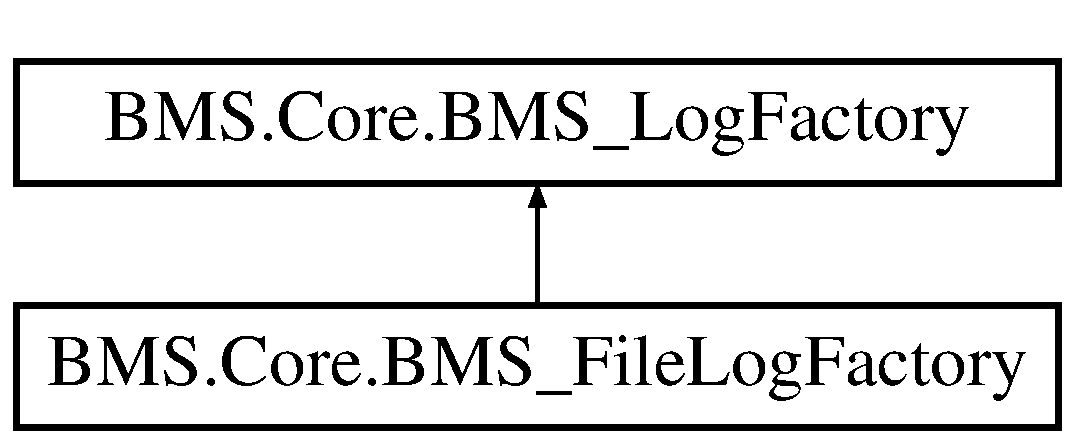
\includegraphics[height=2.000000cm]{class_b_m_s_1_1_core_1_1_b_m_s___file_log_factory}
\end{center}
\end{figure}
\subsection*{Public Member Functions}
\begin{DoxyCompactItemize}
\item 
override \hyperlink{class_b_m_s_1_1_core_1_1_b_m_s___logger}{B\-M\-S\-\_\-\-Logger} \hyperlink{class_b_m_s_1_1_core_1_1_b_m_s___file_log_factory_a84ed51b54cd2ddf8e0af9ccef628ffbe}{create} (string in\-\_\-file\-Name)
\begin{DoxyCompactList}\small\item\em Interface method for \hyperlink{class_b_m_s_1_1_core_1_1_b_m_s___logger}{B\-M\-S\-\_\-\-Logger} object creation \end{DoxyCompactList}\end{DoxyCompactItemize}


\subsection{Member Function Documentation}
\hypertarget{class_b_m_s_1_1_core_1_1_b_m_s___file_log_factory_a84ed51b54cd2ddf8e0af9ccef628ffbe}{\index{B\-M\-S\-::\-Core\-::\-B\-M\-S\-\_\-\-File\-Log\-Factory@{B\-M\-S\-::\-Core\-::\-B\-M\-S\-\_\-\-File\-Log\-Factory}!create@{create}}
\index{create@{create}!BMS::Core::BMS_FileLogFactory@{B\-M\-S\-::\-Core\-::\-B\-M\-S\-\_\-\-File\-Log\-Factory}}
\subsubsection[{create}]{\setlength{\rightskip}{0pt plus 5cm}override {\bf B\-M\-S\-\_\-\-Logger} B\-M\-S.\-Core.\-B\-M\-S\-\_\-\-File\-Log\-Factory.\-create (
\begin{DoxyParamCaption}
\item[{string}]{in\-\_\-file\-Name}
\end{DoxyParamCaption}
)\hspace{0.3cm}{\ttfamily [virtual]}}}\label{class_b_m_s_1_1_core_1_1_b_m_s___file_log_factory_a84ed51b54cd2ddf8e0af9ccef628ffbe}


Interface method for \hyperlink{class_b_m_s_1_1_core_1_1_b_m_s___logger}{B\-M\-S\-\_\-\-Logger} object creation 

\begin{DoxyReturn}{Returns}
A specific \hyperlink{class_b_m_s_1_1_core_1_1_b_m_s___logger}{B\-M\-S\-\_\-\-Logger} subtype as a generic \hyperlink{class_b_m_s_1_1_core_1_1_b_m_s___logger}{B\-M\-S\-\_\-\-Logger}.
\end{DoxyReturn}


Implements \hyperlink{class_b_m_s_1_1_core_1_1_b_m_s___log_factory_aae44a65a49e0f08985f692d180c0931d}{B\-M\-S.\-Core.\-B\-M\-S\-\_\-\-Log\-Factory}.



The documentation for this class was generated from the following file\-:\begin{DoxyCompactItemize}
\item 
E\-:/\-Projects/\-Bad Monkey Software/\-Software/\-B\-M\-E/\-Core/\hyperlink{_b_m_s___file_logger_8cs}{B\-M\-S\-\_\-\-File\-Logger.\-cs}\end{DoxyCompactItemize}

\hypertarget{class_b_m_s_1_1_core_1_1_b_m_s___file_logger}{\section{B\-M\-S.\-Core.\-B\-M\-S\-\_\-\-File\-Logger Class Reference}
\label{class_b_m_s_1_1_core_1_1_b_m_s___file_logger}\index{B\-M\-S.\-Core.\-B\-M\-S\-\_\-\-File\-Logger@{B\-M\-S.\-Core.\-B\-M\-S\-\_\-\-File\-Logger}}
}
Inheritance diagram for B\-M\-S.\-Core.\-B\-M\-S\-\_\-\-File\-Logger\-:\begin{figure}[H]
\begin{center}
\leavevmode
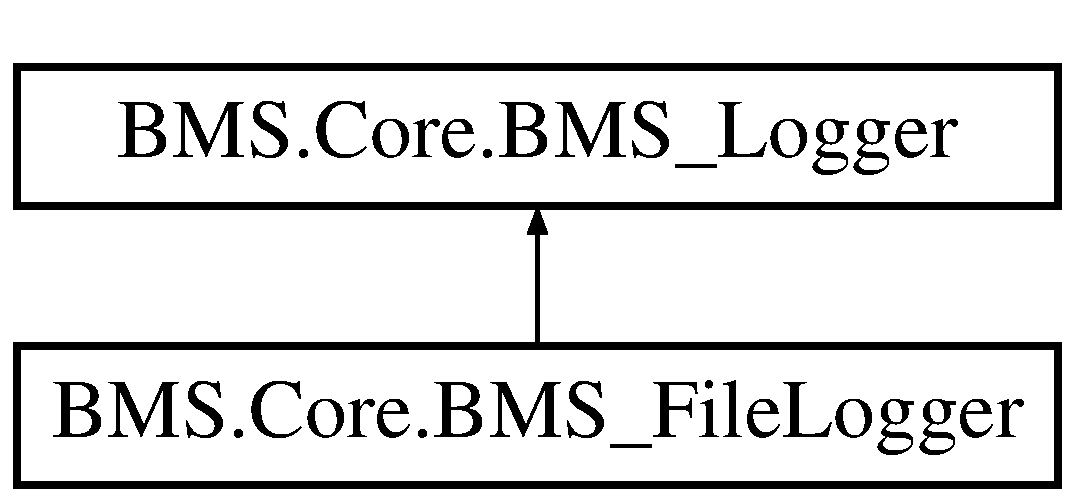
\includegraphics[height=2.000000cm]{class_b_m_s_1_1_core_1_1_b_m_s___file_logger}
\end{center}
\end{figure}
\subsection*{Public Member Functions}
\begin{DoxyCompactItemize}
\item 
\hyperlink{class_b_m_s_1_1_core_1_1_b_m_s___file_logger_a4af5a9f2c7dfb54a63af58073771cf7c}{B\-M\-S\-\_\-\-File\-Logger} ()
\begin{DoxyCompactList}\small\item\em Default constructor. Initializes log level and file location to default values (I\-N\-F\-O and ./log.log) \end{DoxyCompactList}\item 
\hyperlink{class_b_m_s_1_1_core_1_1_b_m_s___file_logger_a35b23ae9c864c71487439c1d23ad3852}{B\-M\-S\-\_\-\-File\-Logger} (string in\-\_\-log\-File\-Name)
\begin{DoxyCompactList}\small\item\em Constructs a \hyperlink{class_b_m_s_1_1_core_1_1_b_m_s___file_logger}{B\-M\-S\-\_\-\-File\-Logger} using the provided log file name and sets the default log level to I\-N\-F\-O \end{DoxyCompactList}\item 
\hyperlink{class_b_m_s_1_1_core_1_1_b_m_s___file_logger_a000dfc0708ec465e275fbb155bd8df26}{B\-M\-S\-\_\-\-File\-Logger} (\hyperlink{namespace_b_m_s_1_1_core_a327c4f5128504a45ef61f00cfd661a43}{e\-Log\-Level} in\-\_\-log\-Lvl, string in\-\_\-log\-File\-Name)
\begin{DoxyCompactList}\small\item\em Constructs a \hyperlink{class_b_m_s_1_1_core_1_1_b_m_s___file_logger}{B\-M\-S\-\_\-\-File\-Logger} using the provided log level and log file name \end{DoxyCompactList}\item 
override void \hyperlink{class_b_m_s_1_1_core_1_1_b_m_s___file_logger_a98aa2f42304a3e323ea5b9991534aa9d}{log} (\hyperlink{namespace_b_m_s_1_1_core_a327c4f5128504a45ef61f00cfd661a43}{e\-Log\-Level} in\-\_\-log\-Lvl, string in\-\_\-message)
\begin{DoxyCompactList}\small\item\em Logs a message to the file log \end{DoxyCompactList}\item 
override void \hyperlink{class_b_m_s_1_1_core_1_1_b_m_s___file_logger_a38541edb5b857325dbd4a2493f5913a1}{set\-Log\-Level} (\hyperlink{namespace_b_m_s_1_1_core_a327c4f5128504a45ef61f00cfd661a43}{e\-Log\-Level} in\-\_\-log\-Lvl)
\begin{DoxyCompactList}\small\item\em Set the current log message filter level for this log \end{DoxyCompactList}\item 
override \hyperlink{namespace_b_m_s_1_1_core_a327c4f5128504a45ef61f00cfd661a43}{e\-Log\-Level} \hyperlink{class_b_m_s_1_1_core_1_1_b_m_s___file_logger_ac0e79bcba3ee49400234b0a01a061dcc}{get\-Log\-Level} ()
\begin{DoxyCompactList}\small\item\em Gets the current log message filter level for this logger \end{DoxyCompactList}\item 
override void \hyperlink{class_b_m_s_1_1_core_1_1_b_m_s___file_logger_ae3a4548c9a583b12773e5c36d3043b87}{set\-Target} (string in\-\_\-log\-Target)
\begin{DoxyCompactList}\small\item\em Sets the file location for this logger. \end{DoxyCompactList}\end{DoxyCompactItemize}
\subsection*{Protected Attributes}
\begin{DoxyCompactItemize}
\item 
string \hyperlink{class_b_m_s_1_1_core_1_1_b_m_s___file_logger_a76f31e7c9e011c718f8c39f987b9d99b}{m\-\_\-file\-U\-R\-I}
\end{DoxyCompactItemize}
\subsection*{Additional Inherited Members}


\subsection{Constructor \& Destructor Documentation}
\hypertarget{class_b_m_s_1_1_core_1_1_b_m_s___file_logger_a4af5a9f2c7dfb54a63af58073771cf7c}{\index{B\-M\-S\-::\-Core\-::\-B\-M\-S\-\_\-\-File\-Logger@{B\-M\-S\-::\-Core\-::\-B\-M\-S\-\_\-\-File\-Logger}!B\-M\-S\-\_\-\-File\-Logger@{B\-M\-S\-\_\-\-File\-Logger}}
\index{B\-M\-S\-\_\-\-File\-Logger@{B\-M\-S\-\_\-\-File\-Logger}!BMS::Core::BMS_FileLogger@{B\-M\-S\-::\-Core\-::\-B\-M\-S\-\_\-\-File\-Logger}}
\subsubsection[{B\-M\-S\-\_\-\-File\-Logger}]{\setlength{\rightskip}{0pt plus 5cm}B\-M\-S.\-Core.\-B\-M\-S\-\_\-\-File\-Logger.\-B\-M\-S\-\_\-\-File\-Logger (
\begin{DoxyParamCaption}
{}
\end{DoxyParamCaption}
)}}\label{class_b_m_s_1_1_core_1_1_b_m_s___file_logger_a4af5a9f2c7dfb54a63af58073771cf7c}


Default constructor. Initializes log level and file location to default values (I\-N\-F\-O and ./log.log) 

\hypertarget{class_b_m_s_1_1_core_1_1_b_m_s___file_logger_a35b23ae9c864c71487439c1d23ad3852}{\index{B\-M\-S\-::\-Core\-::\-B\-M\-S\-\_\-\-File\-Logger@{B\-M\-S\-::\-Core\-::\-B\-M\-S\-\_\-\-File\-Logger}!B\-M\-S\-\_\-\-File\-Logger@{B\-M\-S\-\_\-\-File\-Logger}}
\index{B\-M\-S\-\_\-\-File\-Logger@{B\-M\-S\-\_\-\-File\-Logger}!BMS::Core::BMS_FileLogger@{B\-M\-S\-::\-Core\-::\-B\-M\-S\-\_\-\-File\-Logger}}
\subsubsection[{B\-M\-S\-\_\-\-File\-Logger}]{\setlength{\rightskip}{0pt plus 5cm}B\-M\-S.\-Core.\-B\-M\-S\-\_\-\-File\-Logger.\-B\-M\-S\-\_\-\-File\-Logger (
\begin{DoxyParamCaption}
\item[{string}]{in\-\_\-log\-File\-Name}
\end{DoxyParamCaption}
)}}\label{class_b_m_s_1_1_core_1_1_b_m_s___file_logger_a35b23ae9c864c71487439c1d23ad3852}


Constructs a \hyperlink{class_b_m_s_1_1_core_1_1_b_m_s___file_logger}{B\-M\-S\-\_\-\-File\-Logger} using the provided log file name and sets the default log level to I\-N\-F\-O 


\begin{DoxyParams}{Parameters}
{\em in\-\_\-log\-File\-Name} & The path to the intended log output file.\\
\hline
\end{DoxyParams}
\hypertarget{class_b_m_s_1_1_core_1_1_b_m_s___file_logger_a000dfc0708ec465e275fbb155bd8df26}{\index{B\-M\-S\-::\-Core\-::\-B\-M\-S\-\_\-\-File\-Logger@{B\-M\-S\-::\-Core\-::\-B\-M\-S\-\_\-\-File\-Logger}!B\-M\-S\-\_\-\-File\-Logger@{B\-M\-S\-\_\-\-File\-Logger}}
\index{B\-M\-S\-\_\-\-File\-Logger@{B\-M\-S\-\_\-\-File\-Logger}!BMS::Core::BMS_FileLogger@{B\-M\-S\-::\-Core\-::\-B\-M\-S\-\_\-\-File\-Logger}}
\subsubsection[{B\-M\-S\-\_\-\-File\-Logger}]{\setlength{\rightskip}{0pt plus 5cm}B\-M\-S.\-Core.\-B\-M\-S\-\_\-\-File\-Logger.\-B\-M\-S\-\_\-\-File\-Logger (
\begin{DoxyParamCaption}
\item[{{\bf e\-Log\-Level}}]{in\-\_\-log\-Lvl, }
\item[{string}]{in\-\_\-log\-File\-Name}
\end{DoxyParamCaption}
)}}\label{class_b_m_s_1_1_core_1_1_b_m_s___file_logger_a000dfc0708ec465e275fbb155bd8df26}


Constructs a \hyperlink{class_b_m_s_1_1_core_1_1_b_m_s___file_logger}{B\-M\-S\-\_\-\-File\-Logger} using the provided log level and log file name 


\begin{DoxyParams}{Parameters}
{\em in\-\_\-log\-Lvl} & The desired log level\\
\hline
{\em in\-\_\-log\-File\-Name} & The path to the intended log output file.\\
\hline
\end{DoxyParams}


\subsection{Member Function Documentation}
\hypertarget{class_b_m_s_1_1_core_1_1_b_m_s___file_logger_ac0e79bcba3ee49400234b0a01a061dcc}{\index{B\-M\-S\-::\-Core\-::\-B\-M\-S\-\_\-\-File\-Logger@{B\-M\-S\-::\-Core\-::\-B\-M\-S\-\_\-\-File\-Logger}!get\-Log\-Level@{get\-Log\-Level}}
\index{get\-Log\-Level@{get\-Log\-Level}!BMS::Core::BMS_FileLogger@{B\-M\-S\-::\-Core\-::\-B\-M\-S\-\_\-\-File\-Logger}}
\subsubsection[{get\-Log\-Level}]{\setlength{\rightskip}{0pt plus 5cm}override {\bf e\-Log\-Level} B\-M\-S.\-Core.\-B\-M\-S\-\_\-\-File\-Logger.\-get\-Log\-Level (
\begin{DoxyParamCaption}
{}
\end{DoxyParamCaption}
)\hspace{0.3cm}{\ttfamily [virtual]}}}\label{class_b_m_s_1_1_core_1_1_b_m_s___file_logger_ac0e79bcba3ee49400234b0a01a061dcc}


Gets the current log message filter level for this logger 

\begin{DoxyReturn}{Returns}
The current log filter level.
\end{DoxyReturn}


Implements \hyperlink{class_b_m_s_1_1_core_1_1_b_m_s___logger_ad5812e0e63b7e23ff67d91b14e4af505}{B\-M\-S.\-Core.\-B\-M\-S\-\_\-\-Logger}.

\hypertarget{class_b_m_s_1_1_core_1_1_b_m_s___file_logger_a98aa2f42304a3e323ea5b9991534aa9d}{\index{B\-M\-S\-::\-Core\-::\-B\-M\-S\-\_\-\-File\-Logger@{B\-M\-S\-::\-Core\-::\-B\-M\-S\-\_\-\-File\-Logger}!log@{log}}
\index{log@{log}!BMS::Core::BMS_FileLogger@{B\-M\-S\-::\-Core\-::\-B\-M\-S\-\_\-\-File\-Logger}}
\subsubsection[{log}]{\setlength{\rightskip}{0pt plus 5cm}override void B\-M\-S.\-Core.\-B\-M\-S\-\_\-\-File\-Logger.\-log (
\begin{DoxyParamCaption}
\item[{{\bf e\-Log\-Level}}]{in\-\_\-log\-Lvl, }
\item[{string}]{in\-\_\-message}
\end{DoxyParamCaption}
)\hspace{0.3cm}{\ttfamily [virtual]}}}\label{class_b_m_s_1_1_core_1_1_b_m_s___file_logger_a98aa2f42304a3e323ea5b9991534aa9d}


Logs a message to the file log 


\begin{DoxyParams}{Parameters}
{\em in\-\_\-log\-Lvl} & The log level of this message.\\
\hline
{\em in\-\_\-message} & The message.\\
\hline
\end{DoxyParams}


Implements \hyperlink{class_b_m_s_1_1_core_1_1_b_m_s___logger_a97d054fecacfeb7aadae1f60d35016f2}{B\-M\-S.\-Core.\-B\-M\-S\-\_\-\-Logger}.

\hypertarget{class_b_m_s_1_1_core_1_1_b_m_s___file_logger_a38541edb5b857325dbd4a2493f5913a1}{\index{B\-M\-S\-::\-Core\-::\-B\-M\-S\-\_\-\-File\-Logger@{B\-M\-S\-::\-Core\-::\-B\-M\-S\-\_\-\-File\-Logger}!set\-Log\-Level@{set\-Log\-Level}}
\index{set\-Log\-Level@{set\-Log\-Level}!BMS::Core::BMS_FileLogger@{B\-M\-S\-::\-Core\-::\-B\-M\-S\-\_\-\-File\-Logger}}
\subsubsection[{set\-Log\-Level}]{\setlength{\rightskip}{0pt plus 5cm}override void B\-M\-S.\-Core.\-B\-M\-S\-\_\-\-File\-Logger.\-set\-Log\-Level (
\begin{DoxyParamCaption}
\item[{{\bf e\-Log\-Level}}]{in\-\_\-log\-Lvl}
\end{DoxyParamCaption}
)\hspace{0.3cm}{\ttfamily [virtual]}}}\label{class_b_m_s_1_1_core_1_1_b_m_s___file_logger_a38541edb5b857325dbd4a2493f5913a1}


Set the current log message filter level for this log 


\begin{DoxyParams}{Parameters}
{\em in\-\_\-log\-Lvl} & The new log level.\\
\hline
\end{DoxyParams}


Implements \hyperlink{class_b_m_s_1_1_core_1_1_b_m_s___logger_a5d81080fcbf80bb7246284a725b78cf6}{B\-M\-S.\-Core.\-B\-M\-S\-\_\-\-Logger}.

\hypertarget{class_b_m_s_1_1_core_1_1_b_m_s___file_logger_ae3a4548c9a583b12773e5c36d3043b87}{\index{B\-M\-S\-::\-Core\-::\-B\-M\-S\-\_\-\-File\-Logger@{B\-M\-S\-::\-Core\-::\-B\-M\-S\-\_\-\-File\-Logger}!set\-Target@{set\-Target}}
\index{set\-Target@{set\-Target}!BMS::Core::BMS_FileLogger@{B\-M\-S\-::\-Core\-::\-B\-M\-S\-\_\-\-File\-Logger}}
\subsubsection[{set\-Target}]{\setlength{\rightskip}{0pt plus 5cm}override void B\-M\-S.\-Core.\-B\-M\-S\-\_\-\-File\-Logger.\-set\-Target (
\begin{DoxyParamCaption}
\item[{string}]{in\-\_\-log\-Target}
\end{DoxyParamCaption}
)\hspace{0.3cm}{\ttfamily [virtual]}}}\label{class_b_m_s_1_1_core_1_1_b_m_s___file_logger_ae3a4548c9a583b12773e5c36d3043b87}


Sets the file location for this logger. 


\begin{DoxyParams}{Parameters}
{\em in\-\_\-log\-Target} & The new log target as a file path.\\
\hline
\end{DoxyParams}


Implements \hyperlink{class_b_m_s_1_1_core_1_1_b_m_s___logger_af494d7578070ae9b6d779c9ecc0392d7}{B\-M\-S.\-Core.\-B\-M\-S\-\_\-\-Logger}.



\subsection{Member Data Documentation}
\hypertarget{class_b_m_s_1_1_core_1_1_b_m_s___file_logger_a76f31e7c9e011c718f8c39f987b9d99b}{\index{B\-M\-S\-::\-Core\-::\-B\-M\-S\-\_\-\-File\-Logger@{B\-M\-S\-::\-Core\-::\-B\-M\-S\-\_\-\-File\-Logger}!m\-\_\-file\-U\-R\-I@{m\-\_\-file\-U\-R\-I}}
\index{m\-\_\-file\-U\-R\-I@{m\-\_\-file\-U\-R\-I}!BMS::Core::BMS_FileLogger@{B\-M\-S\-::\-Core\-::\-B\-M\-S\-\_\-\-File\-Logger}}
\subsubsection[{m\-\_\-file\-U\-R\-I}]{\setlength{\rightskip}{0pt plus 5cm}string B\-M\-S.\-Core.\-B\-M\-S\-\_\-\-File\-Logger.\-m\-\_\-file\-U\-R\-I\hspace{0.3cm}{\ttfamily [protected]}}}\label{class_b_m_s_1_1_core_1_1_b_m_s___file_logger_a76f31e7c9e011c718f8c39f987b9d99b}


The documentation for this class was generated from the following file\-:\begin{DoxyCompactItemize}
\item 
E\-:/\-Projects/\-Bad Monkey Software/\-Software/\-B\-M\-E/\-Core/\hyperlink{_b_m_s___file_logger_8cs}{B\-M\-S\-\_\-\-File\-Logger.\-cs}\end{DoxyCompactItemize}

\hypertarget{class_b_m_s_1_1_core_1_1_b_m_s___log_factory}{\section{B\-M\-S.\-Core.\-B\-M\-S\-\_\-\-Log\-Factory Class Reference}
\label{class_b_m_s_1_1_core_1_1_b_m_s___log_factory}\index{B\-M\-S.\-Core.\-B\-M\-S\-\_\-\-Log\-Factory@{B\-M\-S.\-Core.\-B\-M\-S\-\_\-\-Log\-Factory}}
}


Abstract base class for all \hyperlink{class_b_m_s_1_1_core_1_1_b_m_s___log_factory}{B\-M\-S\-\_\-\-Log\-Factory} implementations. Provides interface methods.  


Inheritance diagram for B\-M\-S.\-Core.\-B\-M\-S\-\_\-\-Log\-Factory\-:\begin{figure}[H]
\begin{center}
\leavevmode
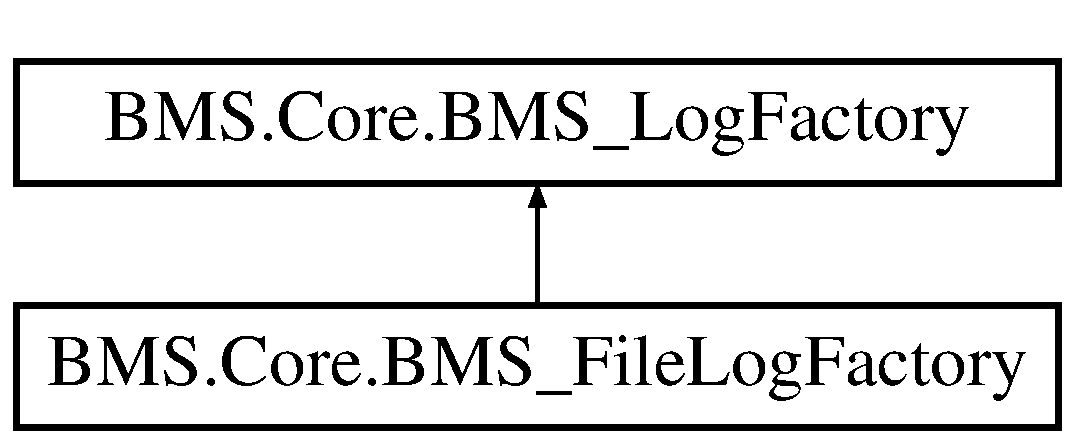
\includegraphics[height=2.000000cm]{class_b_m_s_1_1_core_1_1_b_m_s___log_factory}
\end{center}
\end{figure}
\subsection*{Public Member Functions}
\begin{DoxyCompactItemize}
\item 
abstract \hyperlink{class_b_m_s_1_1_core_1_1_b_m_s___logger}{B\-M\-S\-\_\-\-Logger} \hyperlink{class_b_m_s_1_1_core_1_1_b_m_s___log_factory_aae44a65a49e0f08985f692d180c0931d}{create} (string in\-\_\-file\-Name)
\begin{DoxyCompactList}\small\item\em Interface method for \hyperlink{class_b_m_s_1_1_core_1_1_b_m_s___logger}{B\-M\-S\-\_\-\-Logger} object creation \end{DoxyCompactList}\end{DoxyCompactItemize}


\subsection{Detailed Description}
Abstract base class for all \hyperlink{class_b_m_s_1_1_core_1_1_b_m_s___log_factory}{B\-M\-S\-\_\-\-Log\-Factory} implementations. Provides interface methods. 



\subsection{Member Function Documentation}
\hypertarget{class_b_m_s_1_1_core_1_1_b_m_s___log_factory_aae44a65a49e0f08985f692d180c0931d}{\index{B\-M\-S\-::\-Core\-::\-B\-M\-S\-\_\-\-Log\-Factory@{B\-M\-S\-::\-Core\-::\-B\-M\-S\-\_\-\-Log\-Factory}!create@{create}}
\index{create@{create}!BMS::Core::BMS_LogFactory@{B\-M\-S\-::\-Core\-::\-B\-M\-S\-\_\-\-Log\-Factory}}
\subsubsection[{create}]{\setlength{\rightskip}{0pt plus 5cm}abstract {\bf B\-M\-S\-\_\-\-Logger} B\-M\-S.\-Core.\-B\-M\-S\-\_\-\-Log\-Factory.\-create (
\begin{DoxyParamCaption}
\item[{string}]{in\-\_\-file\-Name}
\end{DoxyParamCaption}
)\hspace{0.3cm}{\ttfamily [pure virtual]}}}\label{class_b_m_s_1_1_core_1_1_b_m_s___log_factory_aae44a65a49e0f08985f692d180c0931d}


Interface method for \hyperlink{class_b_m_s_1_1_core_1_1_b_m_s___logger}{B\-M\-S\-\_\-\-Logger} object creation 

\begin{DoxyReturn}{Returns}
A specific \hyperlink{class_b_m_s_1_1_core_1_1_b_m_s___logger}{B\-M\-S\-\_\-\-Logger} subtype as a generic \hyperlink{class_b_m_s_1_1_core_1_1_b_m_s___logger}{B\-M\-S\-\_\-\-Logger}.
\end{DoxyReturn}


Implemented in \hyperlink{class_b_m_s_1_1_core_1_1_b_m_s___file_log_factory_a84ed51b54cd2ddf8e0af9ccef628ffbe}{B\-M\-S.\-Core.\-B\-M\-S\-\_\-\-File\-Log\-Factory}.



The documentation for this class was generated from the following file\-:\begin{DoxyCompactItemize}
\item 
E\-:/\-Projects/\-Bad Monkey Software/\-Software/\-B\-M\-E/\-Core/\hyperlink{_b_m_s___logger_8cs}{B\-M\-S\-\_\-\-Logger.\-cs}\end{DoxyCompactItemize}

\hypertarget{class_b_m_s_1_1_core_1_1_b_m_s___logger}{\section{B\-M\-S.\-Core.\-B\-M\-S\-\_\-\-Logger Class Reference}
\label{class_b_m_s_1_1_core_1_1_b_m_s___logger}\index{B\-M\-S.\-Core.\-B\-M\-S\-\_\-\-Logger@{B\-M\-S.\-Core.\-B\-M\-S\-\_\-\-Logger}}
}


Abstract base class for all \hyperlink{class_b_m_s_1_1_core_1_1_b_m_s___logger}{B\-M\-S\-\_\-\-Logger} implementations. Provides interface details and common members as well as current logger containers.  


Inheritance diagram for B\-M\-S.\-Core.\-B\-M\-S\-\_\-\-Logger\-:\begin{figure}[H]
\begin{center}
\leavevmode
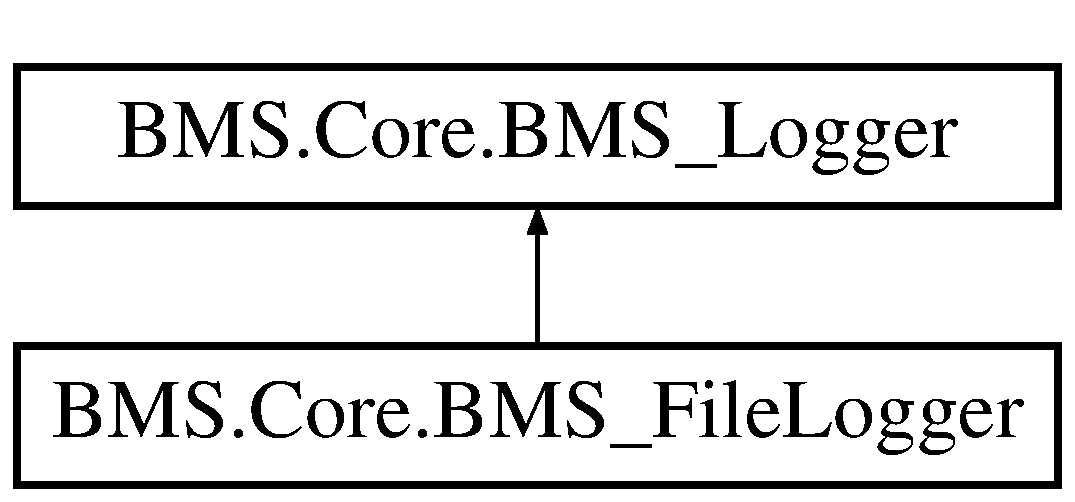
\includegraphics[height=2.000000cm]{class_b_m_s_1_1_core_1_1_b_m_s___logger}
\end{center}
\end{figure}
\subsection*{Public Member Functions}
\begin{DoxyCompactItemize}
\item 
abstract void \hyperlink{class_b_m_s_1_1_core_1_1_b_m_s___logger_a97d054fecacfeb7aadae1f60d35016f2}{log} (\hyperlink{namespace_b_m_s_1_1_core_a327c4f5128504a45ef61f00cfd661a43}{e\-Log\-Level} in\-\_\-log\-Lvl, string in\-\_\-message)
\begin{DoxyCompactList}\small\item\em Interface for writting a message to the log instance \end{DoxyCompactList}\item 
abstract void \hyperlink{class_b_m_s_1_1_core_1_1_b_m_s___logger_a5d81080fcbf80bb7246284a725b78cf6}{set\-Log\-Level} (\hyperlink{namespace_b_m_s_1_1_core_a327c4f5128504a45ef61f00cfd661a43}{e\-Log\-Level} in\-\_\-log\-Lvl)
\begin{DoxyCompactList}\small\item\em Interface to set the log message filter level for the log instance \end{DoxyCompactList}\item 
abstract \hyperlink{namespace_b_m_s_1_1_core_a327c4f5128504a45ef61f00cfd661a43}{e\-Log\-Level} \hyperlink{class_b_m_s_1_1_core_1_1_b_m_s___logger_ad5812e0e63b7e23ff67d91b14e4af505}{get\-Log\-Level} ()
\begin{DoxyCompactList}\small\item\em Interface to get the current log message filter level for the log isntance \end{DoxyCompactList}\item 
abstract void \hyperlink{class_b_m_s_1_1_core_1_1_b_m_s___logger_af494d7578070ae9b6d779c9ecc0392d7}{set\-Target} (string in\-\_\-log\-Target)
\begin{DoxyCompactList}\small\item\em Interface to set the log instance's target (specific per log type) \end{DoxyCompactList}\end{DoxyCompactItemize}
\subsection*{Static Public Member Functions}
\begin{DoxyCompactItemize}
\item 
static \hyperlink{class_b_m_s_1_1_core_1_1_b_m_s___logger}{B\-M\-S\-\_\-\-Logger} \hyperlink{class_b_m_s_1_1_core_1_1_b_m_s___logger_a421d2ae8901e8f936fb51dd71c1e1e32}{get\-Logger} (string in\-\_\-log\-Name)
\begin{DoxyCompactList}\small\item\em Gets the named file logger or creates it if it does not exist \end{DoxyCompactList}\item 
static \hyperlink{class_b_m_s_1_1_core_1_1_b_m_s___logger}{B\-M\-S\-\_\-\-Logger} \hyperlink{class_b_m_s_1_1_core_1_1_b_m_s___logger_afd14fb9faa2e832bda16a5a5f7df41f1}{get\-Logger} (string in\-\_\-log\-Name, \hyperlink{class_b_m_s_1_1_core_1_1_b_m_s___log_factory}{B\-M\-S\-\_\-\-Log\-Factory} in\-\_\-factory)
\begin{DoxyCompactList}\small\item\em Gets the named logger if it exists or creates the logger with the provided log factory. \end{DoxyCompactList}\item 
static void \hyperlink{class_b_m_s_1_1_core_1_1_b_m_s___logger_aa1806fcef246153a42044f6afcb75177}{broadcast} (\hyperlink{namespace_b_m_s_1_1_core_a327c4f5128504a45ef61f00cfd661a43}{e\-Log\-Level} in\-\_\-log\-Lvl, string in\-\_\-message)
\begin{DoxyCompactList}\small\item\em Global log write method. writes the message to all contained (previously created) logs \end{DoxyCompactList}\end{DoxyCompactItemize}
\subsection*{Static Protected Member Functions}
\begin{DoxyCompactItemize}
\item 
static string \hyperlink{class_b_m_s_1_1_core_1_1_b_m_s___logger_a8abcf123f46bba68e51a222c0181a76c}{get\-Time\-Stamp} ()
\begin{DoxyCompactList}\small\item\em Returns a properly formatted time stamp for each log message \end{DoxyCompactList}\item 
static string \hyperlink{class_b_m_s_1_1_core_1_1_b_m_s___logger_a994ce67c23c15d7d52321ede3ff28f64}{get\-Level\-Tag} (\hyperlink{namespace_b_m_s_1_1_core_a327c4f5128504a45ef61f00cfd661a43}{e\-Log\-Level} in\-\_\-log\-Lvl)
\begin{DoxyCompactList}\small\item\em Provides the string representation of the provided log level \end{DoxyCompactList}\end{DoxyCompactItemize}
\subsection*{Protected Attributes}
\begin{DoxyCompactItemize}
\item 
\hyperlink{namespace_b_m_s_1_1_core_a327c4f5128504a45ef61f00cfd661a43}{e\-Log\-Level} \hyperlink{class_b_m_s_1_1_core_1_1_b_m_s___logger_a2a89bc725b72e530c7cb1d8ceb44e74c}{m\-\_\-cur\-Log\-Level}
\begin{DoxyCompactList}\small\item\em The current logger's message filter level \end{DoxyCompactList}\end{DoxyCompactItemize}


\subsection{Detailed Description}
Abstract base class for all \hyperlink{class_b_m_s_1_1_core_1_1_b_m_s___logger}{B\-M\-S\-\_\-\-Logger} implementations. Provides interface details and common members as well as current logger containers. 



\subsection{Member Function Documentation}
\hypertarget{class_b_m_s_1_1_core_1_1_b_m_s___logger_aa1806fcef246153a42044f6afcb75177}{\index{B\-M\-S\-::\-Core\-::\-B\-M\-S\-\_\-\-Logger@{B\-M\-S\-::\-Core\-::\-B\-M\-S\-\_\-\-Logger}!broadcast@{broadcast}}
\index{broadcast@{broadcast}!BMS::Core::BMS_Logger@{B\-M\-S\-::\-Core\-::\-B\-M\-S\-\_\-\-Logger}}
\subsubsection[{broadcast}]{\setlength{\rightskip}{0pt plus 5cm}static void B\-M\-S.\-Core.\-B\-M\-S\-\_\-\-Logger.\-broadcast (
\begin{DoxyParamCaption}
\item[{{\bf e\-Log\-Level}}]{in\-\_\-log\-Lvl, }
\item[{string}]{in\-\_\-message}
\end{DoxyParamCaption}
)\hspace{0.3cm}{\ttfamily [static]}}}\label{class_b_m_s_1_1_core_1_1_b_m_s___logger_aa1806fcef246153a42044f6afcb75177}


Global log write method. writes the message to all contained (previously created) logs 


\begin{DoxyParams}{Parameters}
{\em in\-\_\-log\-Lvl} & The level of this message.\\
\hline
{\em in\-\_\-message} & The message to log.\\
\hline
\end{DoxyParams}
\hypertarget{class_b_m_s_1_1_core_1_1_b_m_s___logger_a994ce67c23c15d7d52321ede3ff28f64}{\index{B\-M\-S\-::\-Core\-::\-B\-M\-S\-\_\-\-Logger@{B\-M\-S\-::\-Core\-::\-B\-M\-S\-\_\-\-Logger}!get\-Level\-Tag@{get\-Level\-Tag}}
\index{get\-Level\-Tag@{get\-Level\-Tag}!BMS::Core::BMS_Logger@{B\-M\-S\-::\-Core\-::\-B\-M\-S\-\_\-\-Logger}}
\subsubsection[{get\-Level\-Tag}]{\setlength{\rightskip}{0pt plus 5cm}static string B\-M\-S.\-Core.\-B\-M\-S\-\_\-\-Logger.\-get\-Level\-Tag (
\begin{DoxyParamCaption}
\item[{{\bf e\-Log\-Level}}]{in\-\_\-log\-Lvl}
\end{DoxyParamCaption}
)\hspace{0.3cm}{\ttfamily [static]}, {\ttfamily [protected]}}}\label{class_b_m_s_1_1_core_1_1_b_m_s___logger_a994ce67c23c15d7d52321ede3ff28f64}


Provides the string representation of the provided log level 


\begin{DoxyParams}{Parameters}
{\em in\-\_\-log\-Lvl} & The log message filter level value to convert.\\
\hline
\end{DoxyParams}
\begin{DoxyReturn}{Returns}
String representation of the filter level value
\end{DoxyReturn}
\hypertarget{class_b_m_s_1_1_core_1_1_b_m_s___logger_a421d2ae8901e8f936fb51dd71c1e1e32}{\index{B\-M\-S\-::\-Core\-::\-B\-M\-S\-\_\-\-Logger@{B\-M\-S\-::\-Core\-::\-B\-M\-S\-\_\-\-Logger}!get\-Logger@{get\-Logger}}
\index{get\-Logger@{get\-Logger}!BMS::Core::BMS_Logger@{B\-M\-S\-::\-Core\-::\-B\-M\-S\-\_\-\-Logger}}
\subsubsection[{get\-Logger}]{\setlength{\rightskip}{0pt plus 5cm}static {\bf B\-M\-S\-\_\-\-Logger} B\-M\-S.\-Core.\-B\-M\-S\-\_\-\-Logger.\-get\-Logger (
\begin{DoxyParamCaption}
\item[{string}]{in\-\_\-log\-Name}
\end{DoxyParamCaption}
)\hspace{0.3cm}{\ttfamily [static]}}}\label{class_b_m_s_1_1_core_1_1_b_m_s___logger_a421d2ae8901e8f936fb51dd71c1e1e32}


Gets the named file logger or creates it if it does not exist 


\begin{DoxyParams}{Parameters}
{\em in\-\_\-log\-Name} & The name of the desired log (access key)\\
\hline
\end{DoxyParams}
\begin{DoxyReturn}{Returns}
The requested file logger
\end{DoxyReturn}
\hypertarget{class_b_m_s_1_1_core_1_1_b_m_s___logger_afd14fb9faa2e832bda16a5a5f7df41f1}{\index{B\-M\-S\-::\-Core\-::\-B\-M\-S\-\_\-\-Logger@{B\-M\-S\-::\-Core\-::\-B\-M\-S\-\_\-\-Logger}!get\-Logger@{get\-Logger}}
\index{get\-Logger@{get\-Logger}!BMS::Core::BMS_Logger@{B\-M\-S\-::\-Core\-::\-B\-M\-S\-\_\-\-Logger}}
\subsubsection[{get\-Logger}]{\setlength{\rightskip}{0pt plus 5cm}static {\bf B\-M\-S\-\_\-\-Logger} B\-M\-S.\-Core.\-B\-M\-S\-\_\-\-Logger.\-get\-Logger (
\begin{DoxyParamCaption}
\item[{string}]{in\-\_\-log\-Name, }
\item[{{\bf B\-M\-S\-\_\-\-Log\-Factory}}]{in\-\_\-factory}
\end{DoxyParamCaption}
)\hspace{0.3cm}{\ttfamily [static]}}}\label{class_b_m_s_1_1_core_1_1_b_m_s___logger_afd14fb9faa2e832bda16a5a5f7df41f1}


Gets the named logger if it exists or creates the logger with the provided log factory. 


\begin{DoxyParams}{Parameters}
{\em in\-\_\-log\-Name} & The name of the desired log\\
\hline
{\em in\-\_\-factory} & The instance of the \hyperlink{class_b_m_s_1_1_core_1_1_b_m_s___log_factory}{B\-M\-S\-\_\-\-Log\-Factory} to use for creation if necessary\\
\hline
\end{DoxyParams}
\begin{DoxyReturn}{Returns}
The requested Logger.
\end{DoxyReturn}
\hypertarget{class_b_m_s_1_1_core_1_1_b_m_s___logger_ad5812e0e63b7e23ff67d91b14e4af505}{\index{B\-M\-S\-::\-Core\-::\-B\-M\-S\-\_\-\-Logger@{B\-M\-S\-::\-Core\-::\-B\-M\-S\-\_\-\-Logger}!get\-Log\-Level@{get\-Log\-Level}}
\index{get\-Log\-Level@{get\-Log\-Level}!BMS::Core::BMS_Logger@{B\-M\-S\-::\-Core\-::\-B\-M\-S\-\_\-\-Logger}}
\subsubsection[{get\-Log\-Level}]{\setlength{\rightskip}{0pt plus 5cm}abstract {\bf e\-Log\-Level} B\-M\-S.\-Core.\-B\-M\-S\-\_\-\-Logger.\-get\-Log\-Level (
\begin{DoxyParamCaption}
{}
\end{DoxyParamCaption}
)\hspace{0.3cm}{\ttfamily [pure virtual]}}}\label{class_b_m_s_1_1_core_1_1_b_m_s___logger_ad5812e0e63b7e23ff67d91b14e4af505}


Interface to get the current log message filter level for the log isntance 

\begin{DoxyReturn}{Returns}
The current log level.
\end{DoxyReturn}


Implemented in \hyperlink{class_b_m_s_1_1_core_1_1_b_m_s___file_logger_ac0e79bcba3ee49400234b0a01a061dcc}{B\-M\-S.\-Core.\-B\-M\-S\-\_\-\-File\-Logger}.

\hypertarget{class_b_m_s_1_1_core_1_1_b_m_s___logger_a8abcf123f46bba68e51a222c0181a76c}{\index{B\-M\-S\-::\-Core\-::\-B\-M\-S\-\_\-\-Logger@{B\-M\-S\-::\-Core\-::\-B\-M\-S\-\_\-\-Logger}!get\-Time\-Stamp@{get\-Time\-Stamp}}
\index{get\-Time\-Stamp@{get\-Time\-Stamp}!BMS::Core::BMS_Logger@{B\-M\-S\-::\-Core\-::\-B\-M\-S\-\_\-\-Logger}}
\subsubsection[{get\-Time\-Stamp}]{\setlength{\rightskip}{0pt plus 5cm}static string B\-M\-S.\-Core.\-B\-M\-S\-\_\-\-Logger.\-get\-Time\-Stamp (
\begin{DoxyParamCaption}
{}
\end{DoxyParamCaption}
)\hspace{0.3cm}{\ttfamily [static]}, {\ttfamily [protected]}}}\label{class_b_m_s_1_1_core_1_1_b_m_s___logger_a8abcf123f46bba68e51a222c0181a76c}


Returns a properly formatted time stamp for each log message 

\begin{DoxyReturn}{Returns}
String representation of the current time stamp.
\end{DoxyReturn}
\hypertarget{class_b_m_s_1_1_core_1_1_b_m_s___logger_a97d054fecacfeb7aadae1f60d35016f2}{\index{B\-M\-S\-::\-Core\-::\-B\-M\-S\-\_\-\-Logger@{B\-M\-S\-::\-Core\-::\-B\-M\-S\-\_\-\-Logger}!log@{log}}
\index{log@{log}!BMS::Core::BMS_Logger@{B\-M\-S\-::\-Core\-::\-B\-M\-S\-\_\-\-Logger}}
\subsubsection[{log}]{\setlength{\rightskip}{0pt plus 5cm}abstract void B\-M\-S.\-Core.\-B\-M\-S\-\_\-\-Logger.\-log (
\begin{DoxyParamCaption}
\item[{{\bf e\-Log\-Level}}]{in\-\_\-log\-Lvl, }
\item[{string}]{in\-\_\-message}
\end{DoxyParamCaption}
)\hspace{0.3cm}{\ttfamily [pure virtual]}}}\label{class_b_m_s_1_1_core_1_1_b_m_s___logger_a97d054fecacfeb7aadae1f60d35016f2}


Interface for writting a message to the log instance 


\begin{DoxyParams}{Parameters}
{\em in\-\_\-log\-Lvl} & The level of this message.\\
\hline
{\em in\-\_\-message} & The message to log.\\
\hline
\end{DoxyParams}


Implemented in \hyperlink{class_b_m_s_1_1_core_1_1_b_m_s___file_logger_a98aa2f42304a3e323ea5b9991534aa9d}{B\-M\-S.\-Core.\-B\-M\-S\-\_\-\-File\-Logger}.

\hypertarget{class_b_m_s_1_1_core_1_1_b_m_s___logger_a5d81080fcbf80bb7246284a725b78cf6}{\index{B\-M\-S\-::\-Core\-::\-B\-M\-S\-\_\-\-Logger@{B\-M\-S\-::\-Core\-::\-B\-M\-S\-\_\-\-Logger}!set\-Log\-Level@{set\-Log\-Level}}
\index{set\-Log\-Level@{set\-Log\-Level}!BMS::Core::BMS_Logger@{B\-M\-S\-::\-Core\-::\-B\-M\-S\-\_\-\-Logger}}
\subsubsection[{set\-Log\-Level}]{\setlength{\rightskip}{0pt plus 5cm}abstract void B\-M\-S.\-Core.\-B\-M\-S\-\_\-\-Logger.\-set\-Log\-Level (
\begin{DoxyParamCaption}
\item[{{\bf e\-Log\-Level}}]{in\-\_\-log\-Lvl}
\end{DoxyParamCaption}
)\hspace{0.3cm}{\ttfamily [pure virtual]}}}\label{class_b_m_s_1_1_core_1_1_b_m_s___logger_a5d81080fcbf80bb7246284a725b78cf6}


Interface to set the log message filter level for the log instance 


\begin{DoxyParams}{Parameters}
{\em in\-\_\-log\-Lvl} & The new log message filter level.\\
\hline
\end{DoxyParams}


Implemented in \hyperlink{class_b_m_s_1_1_core_1_1_b_m_s___file_logger_a38541edb5b857325dbd4a2493f5913a1}{B\-M\-S.\-Core.\-B\-M\-S\-\_\-\-File\-Logger}.

\hypertarget{class_b_m_s_1_1_core_1_1_b_m_s___logger_af494d7578070ae9b6d779c9ecc0392d7}{\index{B\-M\-S\-::\-Core\-::\-B\-M\-S\-\_\-\-Logger@{B\-M\-S\-::\-Core\-::\-B\-M\-S\-\_\-\-Logger}!set\-Target@{set\-Target}}
\index{set\-Target@{set\-Target}!BMS::Core::BMS_Logger@{B\-M\-S\-::\-Core\-::\-B\-M\-S\-\_\-\-Logger}}
\subsubsection[{set\-Target}]{\setlength{\rightskip}{0pt plus 5cm}abstract void B\-M\-S.\-Core.\-B\-M\-S\-\_\-\-Logger.\-set\-Target (
\begin{DoxyParamCaption}
\item[{string}]{in\-\_\-log\-Target}
\end{DoxyParamCaption}
)\hspace{0.3cm}{\ttfamily [pure virtual]}}}\label{class_b_m_s_1_1_core_1_1_b_m_s___logger_af494d7578070ae9b6d779c9ecc0392d7}


Interface to set the log instance's target (specific per log type) 


\begin{DoxyParams}{Parameters}
{\em in\-\_\-log\-Target} & The new log target.\\
\hline
\end{DoxyParams}


Implemented in \hyperlink{class_b_m_s_1_1_core_1_1_b_m_s___file_logger_ae3a4548c9a583b12773e5c36d3043b87}{B\-M\-S.\-Core.\-B\-M\-S\-\_\-\-File\-Logger}.



\subsection{Member Data Documentation}
\hypertarget{class_b_m_s_1_1_core_1_1_b_m_s___logger_a2a89bc725b72e530c7cb1d8ceb44e74c}{\index{B\-M\-S\-::\-Core\-::\-B\-M\-S\-\_\-\-Logger@{B\-M\-S\-::\-Core\-::\-B\-M\-S\-\_\-\-Logger}!m\-\_\-cur\-Log\-Level@{m\-\_\-cur\-Log\-Level}}
\index{m\-\_\-cur\-Log\-Level@{m\-\_\-cur\-Log\-Level}!BMS::Core::BMS_Logger@{B\-M\-S\-::\-Core\-::\-B\-M\-S\-\_\-\-Logger}}
\subsubsection[{m\-\_\-cur\-Log\-Level}]{\setlength{\rightskip}{0pt plus 5cm}{\bf e\-Log\-Level} B\-M\-S.\-Core.\-B\-M\-S\-\_\-\-Logger.\-m\-\_\-cur\-Log\-Level\hspace{0.3cm}{\ttfamily [protected]}}}\label{class_b_m_s_1_1_core_1_1_b_m_s___logger_a2a89bc725b72e530c7cb1d8ceb44e74c}


The current logger's message filter level 



The documentation for this class was generated from the following file\-:\begin{DoxyCompactItemize}
\item 
E\-:/\-Projects/\-Bad Monkey Software/\-Software/\-B\-M\-E/\-Core/\hyperlink{_b_m_s___logger_8cs}{B\-M\-S\-\_\-\-Logger.\-cs}\end{DoxyCompactItemize}

\chapter{File Documentation}
\hypertarget{_b_m_s___file_logger_8cs}{\section{E\-:/\-Projects/\-Bad Monkey Software/\-Software/\-B\-M\-E/\-Core/\-B\-M\-S\-\_\-\-File\-Logger.cs File Reference}
\label{_b_m_s___file_logger_8cs}\index{E\-:/\-Projects/\-Bad Monkey Software/\-Software/\-B\-M\-E/\-Core/\-B\-M\-S\-\_\-\-File\-Logger.\-cs@{E\-:/\-Projects/\-Bad Monkey Software/\-Software/\-B\-M\-E/\-Core/\-B\-M\-S\-\_\-\-File\-Logger.\-cs}}
}
\subsection*{Classes}
\begin{DoxyCompactItemize}
\item 
class \hyperlink{class_b_m_s_1_1_core_1_1_b_m_s___file_log_factory}{B\-M\-S.\-Core.\-B\-M\-S\-\_\-\-File\-Log\-Factory}
\item 
class \hyperlink{class_b_m_s_1_1_core_1_1_b_m_s___file_logger}{B\-M\-S.\-Core.\-B\-M\-S\-\_\-\-File\-Logger}
\end{DoxyCompactItemize}
\subsection*{Namespaces}
\begin{DoxyCompactItemize}
\item 
package \hyperlink{namespace_b_m_s}{B\-M\-S}
\item 
package \hyperlink{namespace_b_m_s_1_1_core}{B\-M\-S.\-Core}
\end{DoxyCompactItemize}

\hypertarget{_b_m_s___logger_8cs}{\section{E\-:/\-Projects/\-Bad Monkey Software/\-Software/\-B\-M\-E/\-Core/\-B\-M\-S\-\_\-\-Logger.cs File Reference}
\label{_b_m_s___logger_8cs}\index{E\-:/\-Projects/\-Bad Monkey Software/\-Software/\-B\-M\-E/\-Core/\-B\-M\-S\-\_\-\-Logger.\-cs@{E\-:/\-Projects/\-Bad Monkey Software/\-Software/\-B\-M\-E/\-Core/\-B\-M\-S\-\_\-\-Logger.\-cs}}
}
\subsection*{Classes}
\begin{DoxyCompactItemize}
\item 
class \hyperlink{class_b_m_s_1_1_core_1_1_b_m_s___log_factory}{B\-M\-S.\-Core.\-B\-M\-S\-\_\-\-Log\-Factory}
\begin{DoxyCompactList}\small\item\em Abstract base class for all \hyperlink{class_b_m_s_1_1_core_1_1_b_m_s___log_factory}{B\-M\-S\-\_\-\-Log\-Factory} implementations. Provides interface methods. \end{DoxyCompactList}\item 
class \hyperlink{class_b_m_s_1_1_core_1_1_b_m_s___logger}{B\-M\-S.\-Core.\-B\-M\-S\-\_\-\-Logger}
\begin{DoxyCompactList}\small\item\em Abstract base class for all \hyperlink{class_b_m_s_1_1_core_1_1_b_m_s___logger}{B\-M\-S\-\_\-\-Logger} implementations. Provides interface details and common members as well as current logger containers. \end{DoxyCompactList}\end{DoxyCompactItemize}
\subsection*{Namespaces}
\begin{DoxyCompactItemize}
\item 
package \hyperlink{namespace_b_m_s}{B\-M\-S}
\item 
package \hyperlink{namespace_b_m_s_1_1_core}{B\-M\-S.\-Core}
\end{DoxyCompactItemize}
\subsection*{Enumerations}
\begin{DoxyCompactItemize}
\item 
enum \hyperlink{namespace_b_m_s_1_1_core_a327c4f5128504a45ef61f00cfd661a43}{B\-M\-S.\-Core.\-e\-Log\-Level} \{ \\*
\hyperlink{namespace_b_m_s_1_1_core_a327c4f5128504a45ef61f00cfd661a43a2d3e4144aa384b18849ab9a8abad74d6}{B\-M\-S.\-Core.\-e\-Log\-Level.\-T\-R\-A\-C\-E} = 1, 
\hyperlink{namespace_b_m_s_1_1_core_a327c4f5128504a45ef61f00cfd661a43adc30ec20708ef7b0f641ef78b7880a15}{B\-M\-S.\-Core.\-e\-Log\-Level.\-D\-E\-B\-U\-G}, 
\hyperlink{namespace_b_m_s_1_1_core_a327c4f5128504a45ef61f00cfd661a43a551b723eafd6a31d444fcb2f5920fbd3}{B\-M\-S.\-Core.\-e\-Log\-Level.\-I\-N\-F\-O}, 
\hyperlink{namespace_b_m_s_1_1_core_a327c4f5128504a45ef61f00cfd661a43a32bd8a1db2275458673903bdb84cb277}{B\-M\-S.\-Core.\-e\-Log\-Level.\-W\-A\-R\-N}, 
\\*
\hyperlink{namespace_b_m_s_1_1_core_a327c4f5128504a45ef61f00cfd661a43abb1ca97ec761fc37101737ba0aa2e7c5}{B\-M\-S.\-Core.\-e\-Log\-Level.\-E\-R\-R\-O\-R}
 \}
\begin{DoxyCompactList}\small\item\em Log filter level value enum \end{DoxyCompactList}\end{DoxyCompactItemize}

\hypertarget{_debug_2_temporary_generated_file__036_c0_b5_b-1481-4323-8_d20-8_f5_a_d_c_b23_d92_8cs}{\section{E\-:/\-Projects/\-Bad Monkey Software/\-Software/\-B\-M\-E/\-Core/obj/\-Debug/\-Temporary\-Generated\-File\-\_\-036\-C0\-B5\-B-\/1481-\/4323-\/8\-D20-\/8\-F5\-A\-D\-C\-B23\-D92.cs File Reference}
\label{_debug_2_temporary_generated_file__036_c0_b5_b-1481-4323-8_d20-8_f5_a_d_c_b23_d92_8cs}\index{E\-:/\-Projects/\-Bad Monkey Software/\-Software/\-B\-M\-E/\-Core/obj/\-Debug/\-Temporary\-Generated\-File\-\_\-036\-C0\-B5\-B-\/1481-\/4323-\/8\-D20-\/8\-F5\-A\-D\-C\-B23\-D92.\-cs@{E\-:/\-Projects/\-Bad Monkey Software/\-Software/\-B\-M\-E/\-Core/obj/\-Debug/\-Temporary\-Generated\-File\-\_\-036\-C0\-B5\-B-\/1481-\/4323-\/8\-D20-\/8\-F5\-A\-D\-C\-B23\-D92.\-cs}}
}

\hypertarget{_debug_01_documented_2_temporary_generated_file__036_c0_b5_b-1481-4323-8_d20-8_f5_a_d_c_b23_d92_8cs}{\section{E\-:/\-Projects/\-Bad Monkey Software/\-Software/\-B\-M\-E/\-Core/obj/\-Debug Documented/\-Temporary\-Generated\-File\-\_\-036\-C0\-B5\-B-\/1481-\/4323-\/8\-D20-\/8\-F5\-A\-D\-C\-B23\-D92.cs File Reference}
\label{_debug_01_documented_2_temporary_generated_file__036_c0_b5_b-1481-4323-8_d20-8_f5_a_d_c_b23_d92_8cs}\index{E\-:/\-Projects/\-Bad Monkey Software/\-Software/\-B\-M\-E/\-Core/obj/\-Debug Documented/\-Temporary\-Generated\-File\-\_\-036\-C0\-B5\-B-\/1481-\/4323-\/8\-D20-\/8\-F5\-A\-D\-C\-B23\-D92.\-cs@{E\-:/\-Projects/\-Bad Monkey Software/\-Software/\-B\-M\-E/\-Core/obj/\-Debug Documented/\-Temporary\-Generated\-File\-\_\-036\-C0\-B5\-B-\/1481-\/4323-\/8\-D20-\/8\-F5\-A\-D\-C\-B23\-D92.\-cs}}
}

\hypertarget{_documentation_2_temporary_generated_file__036_c0_b5_b-1481-4323-8_d20-8_f5_a_d_c_b23_d92_8cs}{\section{E\-:/\-Projects/\-Bad Monkey Software/\-Software/\-B\-M\-E/\-Core/obj/\-Documentation/\-Temporary\-Generated\-File\-\_\-036\-C0\-B5\-B-\/1481-\/4323-\/8\-D20-\/8\-F5\-A\-D\-C\-B23\-D92.cs File Reference}
\label{_documentation_2_temporary_generated_file__036_c0_b5_b-1481-4323-8_d20-8_f5_a_d_c_b23_d92_8cs}\index{E\-:/\-Projects/\-Bad Monkey Software/\-Software/\-B\-M\-E/\-Core/obj/\-Documentation/\-Temporary\-Generated\-File\-\_\-036\-C0\-B5\-B-\/1481-\/4323-\/8\-D20-\/8\-F5\-A\-D\-C\-B23\-D92.\-cs@{E\-:/\-Projects/\-Bad Monkey Software/\-Software/\-B\-M\-E/\-Core/obj/\-Documentation/\-Temporary\-Generated\-File\-\_\-036\-C0\-B5\-B-\/1481-\/4323-\/8\-D20-\/8\-F5\-A\-D\-C\-B23\-D92.\-cs}}
}

\hypertarget{_release_2_temporary_generated_file__036_c0_b5_b-1481-4323-8_d20-8_f5_a_d_c_b23_d92_8cs}{\section{E\-:/\-Projects/\-Bad Monkey Software/\-Software/\-B\-M\-E/\-Core/obj/\-Release/\-Temporary\-Generated\-File\-\_\-036\-C0\-B5\-B-\/1481-\/4323-\/8\-D20-\/8\-F5\-A\-D\-C\-B23\-D92.cs File Reference}
\label{_release_2_temporary_generated_file__036_c0_b5_b-1481-4323-8_d20-8_f5_a_d_c_b23_d92_8cs}\index{E\-:/\-Projects/\-Bad Monkey Software/\-Software/\-B\-M\-E/\-Core/obj/\-Release/\-Temporary\-Generated\-File\-\_\-036\-C0\-B5\-B-\/1481-\/4323-\/8\-D20-\/8\-F5\-A\-D\-C\-B23\-D92.\-cs@{E\-:/\-Projects/\-Bad Monkey Software/\-Software/\-B\-M\-E/\-Core/obj/\-Release/\-Temporary\-Generated\-File\-\_\-036\-C0\-B5\-B-\/1481-\/4323-\/8\-D20-\/8\-F5\-A\-D\-C\-B23\-D92.\-cs}}
}

\hypertarget{_release_01_documented_2_temporary_generated_file__036_c0_b5_b-1481-4323-8_d20-8_f5_a_d_c_b23_d92_8cs}{\section{E\-:/\-Projects/\-Bad Monkey Software/\-Software/\-B\-M\-E/\-Core/obj/\-Release Documented/\-Temporary\-Generated\-File\-\_\-036\-C0\-B5\-B-\/1481-\/4323-\/8\-D20-\/8\-F5\-A\-D\-C\-B23\-D92.cs File Reference}
\label{_release_01_documented_2_temporary_generated_file__036_c0_b5_b-1481-4323-8_d20-8_f5_a_d_c_b23_d92_8cs}\index{E\-:/\-Projects/\-Bad Monkey Software/\-Software/\-B\-M\-E/\-Core/obj/\-Release Documented/\-Temporary\-Generated\-File\-\_\-036\-C0\-B5\-B-\/1481-\/4323-\/8\-D20-\/8\-F5\-A\-D\-C\-B23\-D92.\-cs@{E\-:/\-Projects/\-Bad Monkey Software/\-Software/\-B\-M\-E/\-Core/obj/\-Release Documented/\-Temporary\-Generated\-File\-\_\-036\-C0\-B5\-B-\/1481-\/4323-\/8\-D20-\/8\-F5\-A\-D\-C\-B23\-D92.\-cs}}
}

\hypertarget{_debug_2_temporary_generated_file__5937a670-0e60-4077-877b-f7221da3dda1_8cs}{\section{E\-:/\-Projects/\-Bad Monkey Software/\-Software/\-B\-M\-E/\-Core/obj/\-Debug/\-Temporary\-Generated\-File\-\_\-5937a670-\/0e60-\/4077-\/877b-\/f7221da3dda1.cs File Reference}
\label{_debug_2_temporary_generated_file__5937a670-0e60-4077-877b-f7221da3dda1_8cs}\index{E\-:/\-Projects/\-Bad Monkey Software/\-Software/\-B\-M\-E/\-Core/obj/\-Debug/\-Temporary\-Generated\-File\-\_\-5937a670-\/0e60-\/4077-\/877b-\/f7221da3dda1.\-cs@{E\-:/\-Projects/\-Bad Monkey Software/\-Software/\-B\-M\-E/\-Core/obj/\-Debug/\-Temporary\-Generated\-File\-\_\-5937a670-\/0e60-\/4077-\/877b-\/f7221da3dda1.\-cs}}
}

\hypertarget{_debug_01_documented_2_temporary_generated_file__5937a670-0e60-4077-877b-f7221da3dda1_8cs}{\section{E\-:/\-Projects/\-Bad Monkey Software/\-Software/\-B\-M\-E/\-Core/obj/\-Debug Documented/\-Temporary\-Generated\-File\-\_\-5937a670-\/0e60-\/4077-\/877b-\/f7221da3dda1.cs File Reference}
\label{_debug_01_documented_2_temporary_generated_file__5937a670-0e60-4077-877b-f7221da3dda1_8cs}\index{E\-:/\-Projects/\-Bad Monkey Software/\-Software/\-B\-M\-E/\-Core/obj/\-Debug Documented/\-Temporary\-Generated\-File\-\_\-5937a670-\/0e60-\/4077-\/877b-\/f7221da3dda1.\-cs@{E\-:/\-Projects/\-Bad Monkey Software/\-Software/\-B\-M\-E/\-Core/obj/\-Debug Documented/\-Temporary\-Generated\-File\-\_\-5937a670-\/0e60-\/4077-\/877b-\/f7221da3dda1.\-cs}}
}

\hypertarget{_documentation_2_temporary_generated_file__5937a670-0e60-4077-877b-f7221da3dda1_8cs}{\section{E\-:/\-Projects/\-Bad Monkey Software/\-Software/\-B\-M\-E/\-Core/obj/\-Documentation/\-Temporary\-Generated\-File\-\_\-5937a670-\/0e60-\/4077-\/877b-\/f7221da3dda1.cs File Reference}
\label{_documentation_2_temporary_generated_file__5937a670-0e60-4077-877b-f7221da3dda1_8cs}\index{E\-:/\-Projects/\-Bad Monkey Software/\-Software/\-B\-M\-E/\-Core/obj/\-Documentation/\-Temporary\-Generated\-File\-\_\-5937a670-\/0e60-\/4077-\/877b-\/f7221da3dda1.\-cs@{E\-:/\-Projects/\-Bad Monkey Software/\-Software/\-B\-M\-E/\-Core/obj/\-Documentation/\-Temporary\-Generated\-File\-\_\-5937a670-\/0e60-\/4077-\/877b-\/f7221da3dda1.\-cs}}
}

\hypertarget{_release_2_temporary_generated_file__5937a670-0e60-4077-877b-f7221da3dda1_8cs}{\section{E\-:/\-Projects/\-Bad Monkey Software/\-Software/\-B\-M\-E/\-Core/obj/\-Release/\-Temporary\-Generated\-File\-\_\-5937a670-\/0e60-\/4077-\/877b-\/f7221da3dda1.cs File Reference}
\label{_release_2_temporary_generated_file__5937a670-0e60-4077-877b-f7221da3dda1_8cs}\index{E\-:/\-Projects/\-Bad Monkey Software/\-Software/\-B\-M\-E/\-Core/obj/\-Release/\-Temporary\-Generated\-File\-\_\-5937a670-\/0e60-\/4077-\/877b-\/f7221da3dda1.\-cs@{E\-:/\-Projects/\-Bad Monkey Software/\-Software/\-B\-M\-E/\-Core/obj/\-Release/\-Temporary\-Generated\-File\-\_\-5937a670-\/0e60-\/4077-\/877b-\/f7221da3dda1.\-cs}}
}

\hypertarget{_release_01_documented_2_temporary_generated_file__5937a670-0e60-4077-877b-f7221da3dda1_8cs}{\section{E\-:/\-Projects/\-Bad Monkey Software/\-Software/\-B\-M\-E/\-Core/obj/\-Release Documented/\-Temporary\-Generated\-File\-\_\-5937a670-\/0e60-\/4077-\/877b-\/f7221da3dda1.cs File Reference}
\label{_release_01_documented_2_temporary_generated_file__5937a670-0e60-4077-877b-f7221da3dda1_8cs}\index{E\-:/\-Projects/\-Bad Monkey Software/\-Software/\-B\-M\-E/\-Core/obj/\-Release Documented/\-Temporary\-Generated\-File\-\_\-5937a670-\/0e60-\/4077-\/877b-\/f7221da3dda1.\-cs@{E\-:/\-Projects/\-Bad Monkey Software/\-Software/\-B\-M\-E/\-Core/obj/\-Release Documented/\-Temporary\-Generated\-File\-\_\-5937a670-\/0e60-\/4077-\/877b-\/f7221da3dda1.\-cs}}
}

\hypertarget{_debug_2_temporary_generated_file___e7_a71_f73-0_f8_d-4_b9_b-_b56_e-8_e70_b10_b_c5_d3_8cs}{\section{E\-:/\-Projects/\-Bad Monkey Software/\-Software/\-B\-M\-E/\-Core/obj/\-Debug/\-Temporary\-Generated\-File\-\_\-\-E7\-A71\-F73-\/0\-F8\-D-\/4\-B9\-B-\/\-B56\-E-\/8\-E70\-B10\-B\-C5\-D3.cs File Reference}
\label{_debug_2_temporary_generated_file___e7_a71_f73-0_f8_d-4_b9_b-_b56_e-8_e70_b10_b_c5_d3_8cs}\index{E\-:/\-Projects/\-Bad Monkey Software/\-Software/\-B\-M\-E/\-Core/obj/\-Debug/\-Temporary\-Generated\-File\-\_\-\-E7\-A71\-F73-\/0\-F8\-D-\/4\-B9\-B-\/\-B56\-E-\/8\-E70\-B10\-B\-C5\-D3.\-cs@{E\-:/\-Projects/\-Bad Monkey Software/\-Software/\-B\-M\-E/\-Core/obj/\-Debug/\-Temporary\-Generated\-File\-\_\-\-E7\-A71\-F73-\/0\-F8\-D-\/4\-B9\-B-\/\-B56\-E-\/8\-E70\-B10\-B\-C5\-D3.\-cs}}
}

\hypertarget{_debug_01_documented_2_temporary_generated_file___e7_a71_f73-0_f8_d-4_b9_b-_b56_e-8_e70_b10_b_c5_d3_8cs}{\section{E\-:/\-Projects/\-Bad Monkey Software/\-Software/\-B\-M\-E/\-Core/obj/\-Debug Documented/\-Temporary\-Generated\-File\-\_\-\-E7\-A71\-F73-\/0\-F8\-D-\/4\-B9\-B-\/\-B56\-E-\/8\-E70\-B10\-B\-C5\-D3.cs File Reference}
\label{_debug_01_documented_2_temporary_generated_file___e7_a71_f73-0_f8_d-4_b9_b-_b56_e-8_e70_b10_b_c5_d3_8cs}\index{E\-:/\-Projects/\-Bad Monkey Software/\-Software/\-B\-M\-E/\-Core/obj/\-Debug Documented/\-Temporary\-Generated\-File\-\_\-\-E7\-A71\-F73-\/0\-F8\-D-\/4\-B9\-B-\/\-B56\-E-\/8\-E70\-B10\-B\-C5\-D3.\-cs@{E\-:/\-Projects/\-Bad Monkey Software/\-Software/\-B\-M\-E/\-Core/obj/\-Debug Documented/\-Temporary\-Generated\-File\-\_\-\-E7\-A71\-F73-\/0\-F8\-D-\/4\-B9\-B-\/\-B56\-E-\/8\-E70\-B10\-B\-C5\-D3.\-cs}}
}

\hypertarget{_documentation_2_temporary_generated_file___e7_a71_f73-0_f8_d-4_b9_b-_b56_e-8_e70_b10_b_c5_d3_8cs}{\section{E\-:/\-Projects/\-Bad Monkey Software/\-Software/\-B\-M\-E/\-Core/obj/\-Documentation/\-Temporary\-Generated\-File\-\_\-\-E7\-A71\-F73-\/0\-F8\-D-\/4\-B9\-B-\/\-B56\-E-\/8\-E70\-B10\-B\-C5\-D3.cs File Reference}
\label{_documentation_2_temporary_generated_file___e7_a71_f73-0_f8_d-4_b9_b-_b56_e-8_e70_b10_b_c5_d3_8cs}\index{E\-:/\-Projects/\-Bad Monkey Software/\-Software/\-B\-M\-E/\-Core/obj/\-Documentation/\-Temporary\-Generated\-File\-\_\-\-E7\-A71\-F73-\/0\-F8\-D-\/4\-B9\-B-\/\-B56\-E-\/8\-E70\-B10\-B\-C5\-D3.\-cs@{E\-:/\-Projects/\-Bad Monkey Software/\-Software/\-B\-M\-E/\-Core/obj/\-Documentation/\-Temporary\-Generated\-File\-\_\-\-E7\-A71\-F73-\/0\-F8\-D-\/4\-B9\-B-\/\-B56\-E-\/8\-E70\-B10\-B\-C5\-D3.\-cs}}
}

\hypertarget{_release_2_temporary_generated_file___e7_a71_f73-0_f8_d-4_b9_b-_b56_e-8_e70_b10_b_c5_d3_8cs}{\section{E\-:/\-Projects/\-Bad Monkey Software/\-Software/\-B\-M\-E/\-Core/obj/\-Release/\-Temporary\-Generated\-File\-\_\-\-E7\-A71\-F73-\/0\-F8\-D-\/4\-B9\-B-\/\-B56\-E-\/8\-E70\-B10\-B\-C5\-D3.cs File Reference}
\label{_release_2_temporary_generated_file___e7_a71_f73-0_f8_d-4_b9_b-_b56_e-8_e70_b10_b_c5_d3_8cs}\index{E\-:/\-Projects/\-Bad Monkey Software/\-Software/\-B\-M\-E/\-Core/obj/\-Release/\-Temporary\-Generated\-File\-\_\-\-E7\-A71\-F73-\/0\-F8\-D-\/4\-B9\-B-\/\-B56\-E-\/8\-E70\-B10\-B\-C5\-D3.\-cs@{E\-:/\-Projects/\-Bad Monkey Software/\-Software/\-B\-M\-E/\-Core/obj/\-Release/\-Temporary\-Generated\-File\-\_\-\-E7\-A71\-F73-\/0\-F8\-D-\/4\-B9\-B-\/\-B56\-E-\/8\-E70\-B10\-B\-C5\-D3.\-cs}}
}

\hypertarget{_release_01_documented_2_temporary_generated_file___e7_a71_f73-0_f8_d-4_b9_b-_b56_e-8_e70_b10_b_c5_d3_8cs}{\section{E\-:/\-Projects/\-Bad Monkey Software/\-Software/\-B\-M\-E/\-Core/obj/\-Release Documented/\-Temporary\-Generated\-File\-\_\-\-E7\-A71\-F73-\/0\-F8\-D-\/4\-B9\-B-\/\-B56\-E-\/8\-E70\-B10\-B\-C5\-D3.cs File Reference}
\label{_release_01_documented_2_temporary_generated_file___e7_a71_f73-0_f8_d-4_b9_b-_b56_e-8_e70_b10_b_c5_d3_8cs}\index{E\-:/\-Projects/\-Bad Monkey Software/\-Software/\-B\-M\-E/\-Core/obj/\-Release Documented/\-Temporary\-Generated\-File\-\_\-\-E7\-A71\-F73-\/0\-F8\-D-\/4\-B9\-B-\/\-B56\-E-\/8\-E70\-B10\-B\-C5\-D3.\-cs@{E\-:/\-Projects/\-Bad Monkey Software/\-Software/\-B\-M\-E/\-Core/obj/\-Release Documented/\-Temporary\-Generated\-File\-\_\-\-E7\-A71\-F73-\/0\-F8\-D-\/4\-B9\-B-\/\-B56\-E-\/8\-E70\-B10\-B\-C5\-D3.\-cs}}
}

\hypertarget{_assembly_info_8cs}{\section{E\-:/\-Projects/\-Bad Monkey Software/\-Software/\-B\-M\-E/\-Core/\-Properties/\-Assembly\-Info.cs File Reference}
\label{_assembly_info_8cs}\index{E\-:/\-Projects/\-Bad Monkey Software/\-Software/\-B\-M\-E/\-Core/\-Properties/\-Assembly\-Info.\-cs@{E\-:/\-Projects/\-Bad Monkey Software/\-Software/\-B\-M\-E/\-Core/\-Properties/\-Assembly\-Info.\-cs}}
}

%--- End generated contents ---

% Index
\newpage
\phantomsection
\addcontentsline{toc}{part}{Index}
\printindex

\end{document}
